\documentclass[a4paper,10pt]{article}

% Paquetes
\usepackage{fontspec}
\usepackage{titlesec}
\usepackage{titling}
\usepackage{setspace}
\usepackage[hidelinks]{hyperref}
\usepackage{graphicx}
\usepackage{caption}
%\usepackage{subcaption}
\usepackage{subfig}
\usepackage{float}
\usepackage{xcolor}
\usepackage[affil-it]{authblk}
\usepackage{multirow}
\usepackage{colortbl}
\usepackage{hyperref}
\usepackage{biblatex}
\addbibresource{nfc.bib}
\usepackage[nottoc]{tocbibind}
\usepackage{adjustbox,lipsum}
\usepackage[margin=1in]{geometry} 
\usepackage{amsmath,amsthm,amssymb}
\usepackage{yhmath}

% Idioma
\usepackage[spanish]{babel}
\usepackage{inputenc}
\usepackage{csquotes}

% Graficos
\usepackage{graphicx}
\graphicspath{ {images/} }
\usepackage{subfig}


% Configuraciones
\setmainfont{Times New Roman}
\hypersetup{
    colorlinks,
    linkcolor={red!50!black},
    citecolor={blue!50!black},
    urlcolor={blue!80!black}
}


\begin{document}
\begin{titlepage}
\centering
\begin{figure}[t]
	\centering
	
\includegraphics[scale=0.15]{utn.jpg}
    \vspace{0.5cm}
\end{figure}%
	{\LARGE Proyecto Final\par}
    {\LARGE 2017\par}
	\vspace{1cm}
	{\huge\bfseries Desarrollo del Frontend Analógico RFID y un Banco de Prueba basado en el estándar ISO-14443\par}
	\vspace{1cm}
    {\LARGE Tesina\par}
    \vspace{1cm}
	{\Large\itshape Yao-Ming Kuo, Agustín Grosso, Flavio Galimberti, Juan Tántera\par}
	\vfill
\end{titlepage}


\tableofcontents


%\newpage
%\section{Objeto del Documento}
%\label{sec:0_objeto}
%Este documento tiene por objeto la explicación  detallada  y  con  el  máximo  rigor  técnico  los conceptos  teóricos  de  aplicación  en  el  proyecto,  con  referencias  bibliográficas  que cubran  los  contenidos  teóricos  clásicos,  la  cual  debe  ser  actualizada  y  de  reconocido prestigio.

\clearpage
\section{Abstract}
\label{sec:abstract}
Éste documento describe el diseño del \textit{Front-End Analógico} (AFE) compuestos por los módulos de rectificación, regulación de tensión, generador de clock, power-on-reset, modulación de carga, y demodulación de un transceptor RFID (13.56 MHz) compatible con la norma ISO/IEC 14443. El AFE se diseñó, simuló y se implementó para dos procesos de fabricación \textit{Complementary metal–oxide–semiconductor} (CMOS): \textbf{Global Foundries 130 nm (GF130)} y \textbf{ON Semiconductor 500 nm (ONC5)}. Los chips se fabricaron a través del programa universitario de \textit{MOSIS}.

Aparte del diseño, también se dará una introducción del marco teórico, las teorías clásicas involucradas y el protocolo de comunicación ISO/IEC14443A.

Además se incluye el diseño de un banco de prueba \textit{(testbench)} con un \textit{FPGA} y la validación de la comunicación con un analizador lógico \textit{Agilent 16806A}.


\section{Introducción}
\label{sec:intro}
\subsection{Tema de investigación}
Debido al creciente desarrollo de productos de RFID en la última década, se comenzó a investigar ésta tecnología con el objetivo de llevar a cabo un desarrollo nacional que pueda utilizarse en múltiples aplicaciones. Se describe en el presente documento el desarrollo de los módulos de rectificación, regulación de tensión, generador de clock, power-on-reset, modulación de carga, y demodulación de un transceptor RFID para los procesos de fabricación con el que cuenta el \textbf{Departamento de Electrónica de la Facultad Regional Buenos Aires}.
El rango de frecuencia utilizado en el proyecto es el de 13,553 a 13,567 MHz (según indica la norma ISO/IEC14443), el cual está situado en el medio del rango de longitud de onda corta del espectro electromagnético.
Se busca presentar los primeros pasos del diseño y desarrollo de un transceptor mediante la tecnología RFID. En el proceso de su desarrollo fue necesario diseñar la antena para la transmisión y recepción de información, el \textit{Front-End} analógico para la comunicación entre el lector \textit{PCD (Proximity Coupling Device)}, la tarjeta \textit{PICC (Proximity Integrated Circuit Card)} y la validación del protocolo de comunicación.

\subsection{Descripción del proyecto}

El grupo de investigación está conformado por 4 estudiantes de la carrera de Ingeniería Electrónica en la Universidad Tecnológica Nacional (Facultad Regional Buenos Aires). La investigación y desarrollo del \textit{Front-End} comenzó en el año 2015 a través de \textit{MOSIS®} en un proceso de fabricación estandar \textit{CMOS} de 500 nm (longitud mínima del canal de transistor).

El proyecto consiste en la puesta en marcha de la parte analógica de un chip transceptor RFID, el desarrollo de la parte digital del protocolo de comunicación bajo la norma ISO/IEC 14443 y por último un banco de prueba para poder verificar el correcto funcionamiento del conjunto analógico y digital con un microcontrolador que a su vez opere bajo la norma antes mencionada.

En la actualidad además del desarrollo en 500nm, también se implementó con la tecnología de 130nm para poder integrar la parte digital del proyecto al chip y además se cuenta con la posibilidad de integrar memorias.

%\subsection{Alcance del proyecto}
%El proyecto consiste en la fabricación, medición y análisis del funcionamiento del Front-End Analógico para los procesos de fabricación \textit{On Semiconductor (500 nm)} y \textit{Global Foundries (130 nm)}.
%También consiste en el armado de una placa discreta que cumpla con las mismas funciones (Modulación, demodulación, generador de clock, power on reset).
%Además se hará un banco de prueba en una \textit{FPGA (Avnet Xilinx SPARTAN 6 LX9 Microboard)} para validar el envío y recepción de los símbolos, cumpliendo la norma \textit{ISO14443-A}. La correcta interpretación de símbolos es muy importante para el funcionamiento del sistema. En lo posible, se contemplará la posibilidad de implementación del protocolo de comunicación. 

\clearpage
\section{Gestión del proyecto}
\label{sec:gestion}
Durante el año de realización de este trabajo para la cátedra de Proyecto Final, se realizó una serie de análisis orientados a la gestión, previsión y orden del proyecto.
En esta sección se muestran los análisis específicos que formaron parte de la gestión del proyecto.



\subsection{Gestión del tiempo}
\label{sec:tiempo}
{\centering
	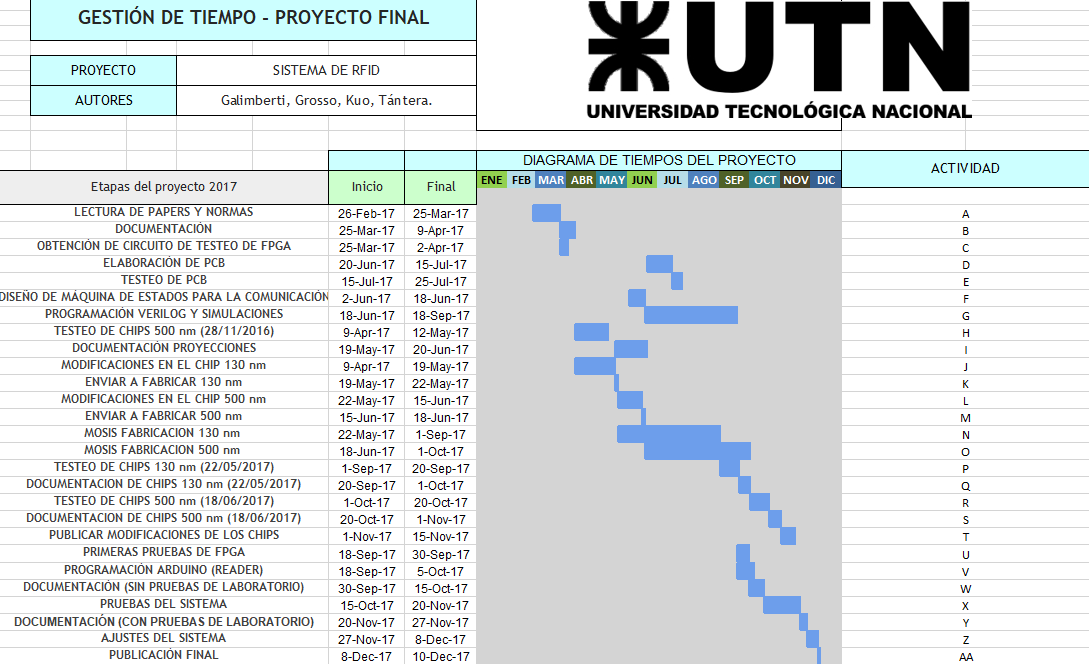
\includegraphics[scale=0.55]{Gestion/GDT.png}
}
\newline
\newline

\label{sec:tiempo}
{\centering
    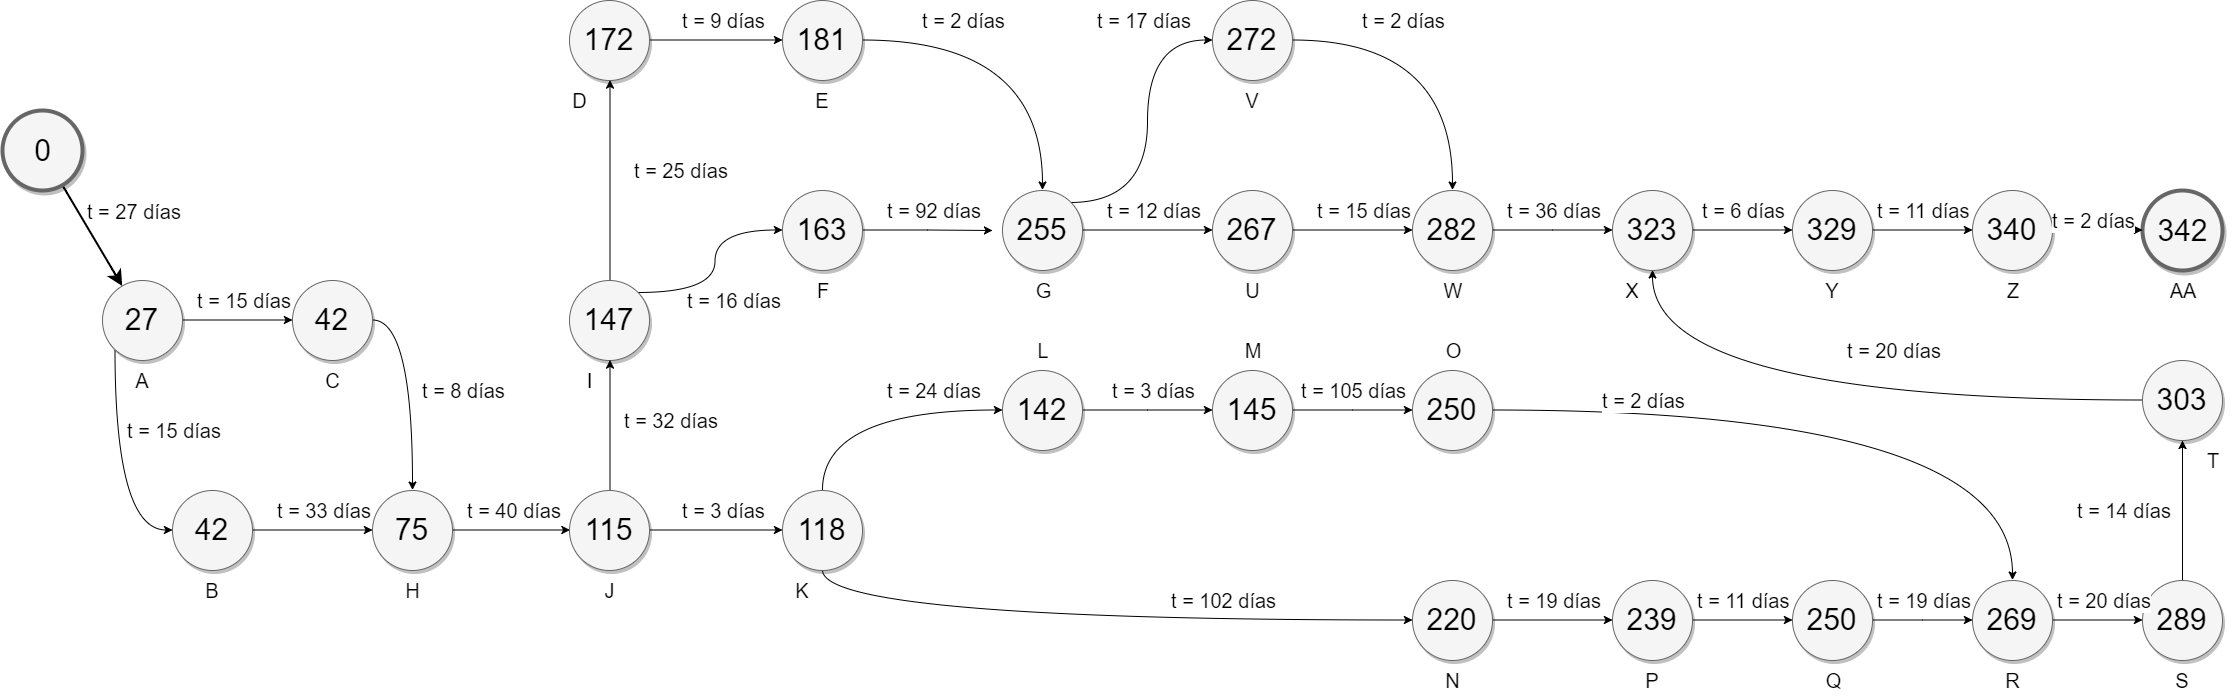
\includegraphics[scale=0.2]{Gestion/diagrama_de_tiempo.png}
}
\newpage
\subsection{Matriz FODA}
\label{sec:FODA}
Analizando el proyecto y las situaciones externas a éste, se procedió al armado de la matriz que refleja: \newline 
- Fortalezas y debilidades internas \newline  
- Oportunidades y amenazas externas \newline
{\centering
	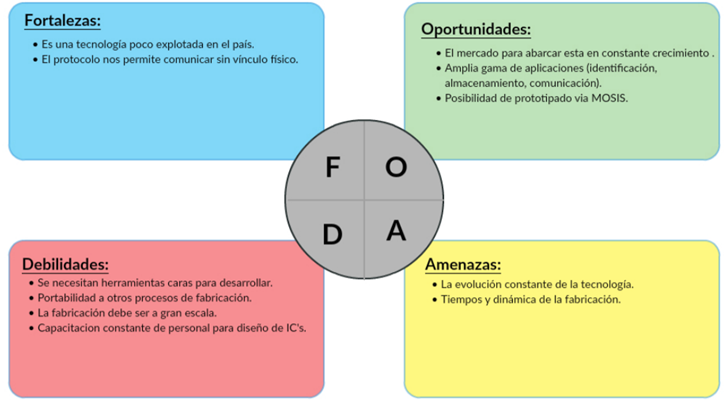
\includegraphics[scale=0.8]{Gestion/FODA.png}
}


\subsection{Gestión de problemas}
\label{sec:problemas}
Como principales problemas podemos detectar 3
\begin{enumerate}
\item No disponer del chip:
	\begin{itemize}
    	\item Dada de baja a la tecnología en la cual se realizó el desarrollo.
		\item Debido a discontinuidad de las corridas por aprte de las foundries (On Semi Conductors 500nm o Global Foundries 130nm).
		\item Debido a retrasos en la entrega de las foundires.
	\end{itemize}
\item No poder realizar modificaciones en el chip:
    \begin{itemize}
    	\item Inconvenientes en el desarrollo y empleo de PDK's.
		\item Que surjan inconvenientes con el uso de las licencias o no poseerlas.
    \end{itemize}
\item Mal funcionamiento del chip
	\begin{itemize}
        \item Dispersiones fuera de rango en la fabricación del mismo. 
	\end{itemize}
\end{enumerate}

\newpage

\subsection{Gestión de objetivos}
\label{sec:objetivos}
En función de los inconvenientes comentados en la gestión de problemas se plantean los siguientes objetivos
\begin{enumerate}
\item Abstracción de variabilidades en foundries:
	\begin{itemize}
    	\item Migración de tecnología (por ejemplo de 500nm a 130nm).
		\item Realizar la corrida actual en varias tecnologías para asegurar una entrega.
		\item Disponibilidad del circuito en discreto.
	\end{itemize}
\item Uso de herramientas confiables:
    \begin{itemize}
    	\item Utilizar los PDK's nativos otorgados por las foundries.
		\item Poseer confiabilidad en el servidor y una correcta configuración del mismo.
    \end{itemize}
\item Disminuir la probabilidad de errores en la fabricación del chip:
	\begin{itemize}
        \item Simulación con corners y metodología "Montecarlo". 
	\end{itemize}
\end{enumerate}

\subsection{Matriz de riesgos}
\label{sec:riesgos}
Análisis del nivel de riesgo de las tareas sobre la realización del proyecto.


\begin{tabular}{|l|r|r|r|r|r|}
\hline \multirow{2}{1.8cm}{PROBABIL.}
& \multicolumn{5}{p{10cm}|}%
{\centering IMPACTO}\tabularnewline \cline{2-6}
& \multicolumn{1}{p{1.7cm}|}%
{\centering MUY BAJO}
& \multicolumn{1}{p{1.7cm}|}%
{\centering BAJO}
& \multicolumn{1}{p{1.7cm}|}%
{\centering MEDIO}
& \multicolumn{1}{p{1.7cm}|}%
{\centering ALTO}
& \multicolumn{1}{p{1.7cm}|}%
{\centering MUY ALTO}

\tabularnewline \hline
MUY ALTA &\cellcolor{yellow}&\cellcolor{orange}&\cellcolor{orange}Interrupción de trabajo&
\cellcolor{red}&\cellcolor{red}\\
&\cellcolor{yellow}&\cellcolor{orange}
&\cellcolor{orange}debido a exámenes&
\cellcolor{red}&\cellcolor{red}\\
\hline
ALTA&\cellcolor{green}
&\cellcolor{yellow}
&\cellcolor{orange}
&\cellcolor{orange}&\cellcolor{red} \\
&\cellcolor{green}&\cellcolor{yellow}
&\cellcolor{orange}&
\cellcolor{orange}&\cellcolor{red}\\   
\hline
MEDIA&\cellcolor{green}&\cellcolor{yellow}Falta de stock
&\cellcolor{yellow}Malfuncionamiento&
\cellcolor{orange}Atraso en entrega de&\cellcolor{orange}Falla de la\\
&\cellcolor{green}&\cellcolor{yellow}de componentes
&\cellcolor{yellow}de placa de test&
\cellcolor{orange}chip&\cellcolor{orange}fabricación \\
\hline
BAJA   &\cellcolor{green}
&\cellcolor{green}Demora en la
&\cellcolor{yellow}Falta de &
\cellcolor{yellow}Malfuncionamiento&\cellcolor{orange} Mal diseño\\
&\cellcolor{green}
&\cellcolor{green}fabric. de placa
&\cellcolor{yellow}documentacion&
\cellcolor{yellow}de FPGA&\cellcolor{orange}del chip\\
\hline
 MUY BAJA   &\cellcolor{green}&\cellcolor{green}&\cellcolor{green}&
 \cellcolor{green}Malfuncionamiento&\cellcolor{yellow}No disponibilidad\\
 &\cellcolor{green}&\cellcolor{green}&\cellcolor{green}
 &\cellcolor{green}de arduino (reader)&\cellcolor{yellow}de herramienta\\
\hline
\end{tabular}



\newpage
\subsection{KPI's}
\label{sec:descripción}
A continuación enunciaremos cómo se conformaron nuestros indicadores y en que valor se encuentran actualmente
\begin{itemize}
\item Hitos Fallidos (HF): Mide el porcentaje de hitos fallidos a tiempo sobre el total de hitos.
	\begin{itemize}
    	\item Tendencia deseada: Negativa.
		\item Periodo de captura: Mes.
		\item Frecuencia de medida: mensual.
	\end{itemize}
\item Retraso del proytecto (RP): Mide el retraso total del proyecto mediante la suma de los retrasos registrados en cada uno de los estados de implementación del proyecto.
	\begin{itemize}
    	\item Tendencia deseada: Negativa.
		\item Periodo de captura: Ejercicio hasta la fecha.
		\item Frecuencia de medida: Mensual.
	\end{itemize}
\item Tareas Atrasadas (TA): Mide el porcenta de tareas retrasadas del número total de tareas actuales.
	\begin{itemize}
    	\item Tendencia deseada: Negativa.
		\item Periodo de captura: Puntual.
		\item Frecuencia de medida: Semanal.
	\end{itemize}
\item Incidencias Identificadas en el Proyecto (IIP): Mide el número de nuevas incidencias que son identificados y necesitan resolverse una vez iniciado el proyecto.
	\begin{itemize}
    	\item Tendencia deseada: Negativa.
		\item Periodo de captura: Semanal.
		\item Frecuencia de medida: Semanal.
	\end{itemize}
\item Riesgos (R): Mide el número de riesgos identificados.
	\begin{itemize}
    	\item Tendencia deseada: Positiva.
		\item Periodo de captura: Puntual.
		\item Frecuencia de medida: Trimestral.
	\end{itemize}
\item Riesgos Posibles (RPo): Mide el porcentaje de riesgos que todavía pueden tener lugar en el momento del proyecto.
	\begin{itemize}
    	\item Tendencia deseada: Negativa.
		\item Periodo de captura: Puntual.
		\item Frecuencia de medida: Mensual.
	\end{itemize}
\item Plazos de Entrega Cumplidos (PEC): Mide el porcentaje de plazos de entrega cumplidos durante el proyecto sobre el total.
	\begin{itemize}
    	\item Tendencia deseada: Negativa.
		\item Periodo de captura: Puntual.
		\item Frecuencia de medida: Mensual.
	\end{itemize}
\end{itemize}

Algunos de los valores que tomaron los KPI's durante el proyecto fueron los siguientes:

\begin{center}
  \begin{tabular}{ | l | c | l |}
    \hline
    KPI & Valor & Detalle \\ \hline
    HF & 3.84\% & Retraso en la finalización del PCB sobre un total de 26 hitos.\\ \hline
    RP & 0.5 &  Medio mes de retraso en la finalización del PCB.\\ \hline
    TA & 14.28\% & Una sola tarea en un total de nueve activas. \\ \hline
	IIP & 1  & Incompatibilidad con ISE. \\ \hline
	R & 2  & Dos de los tres riesgos están latentes al momento, no disponer ni poder modificar el chip.\\ \hline
	RPo & 100\% & Todos los riesgos pueden tener lugar. \\  \hline
    PEC & 94.4\% & Diecisiete de los dieciocho plazos de entrega fueron cumplidos. \\
    \hline
  \end{tabular}
\end{center}




\clearpage
\section{Marco Teórico}
\label{sec:marco}
%\section{Introducción Teórica del tema a tratar y Marco Teórico}
\label{sec:2_marcoteorico}

\subsection{Historia del RFID}

\begin{itemize}
\item \textbf{1860:} James Clerk Maxwell, físico escocés, predijo la existencia de ondas radio y postuló su uso.

\item \textbf{1886:} Un científico alemán, Heinrich Rudolf Hertz probó que rápidas variaciones de corriente 	eléctrica podían ser proyectadas en el espacio en forma de ondas de radio, similar a las ondas de luz, y que ,éstas, eran medibles y repetibles.

\item \textbf{1902:} Guglielmo Marconi, físico italiano, demostró la primera comunicación de larga distancia usando ondas radio, atravesando el Atlántico. Consistió en transmitir SOS en código Morse, en particular la letra S.

\item \textbf{1942 (Durante la II Guerra Mundial):} Los británicos desarrollaron el primer sistema etiquetado de RFID, el objetivo era discriminar rápidamente entre su propia flota de aviones y los escuadrones alemanes. Los aviones británicos incorporaban tags que contestaban a un lector con un código \textit{“I am a friend”}. Basado en el sistema de identificación \textit{IFF (Identity Friend or Foe)}.

\item \textbf{1960:} La necesidad de seguridad en los materiales nucleares condujo al desarrollo de una etiqueta RFID como el EAS \textit{(Electronic Article Surveillance)}.

\item \textbf{1977:} La necesidad de seguridad en los materiales nucleares condujo al desarrollo de una etiqueta RFID como el EAS \textit{(Electronic Article Surveillance)}.

\item \textbf{A partir de 1980:} Se focaliza en la comercialización de la RFID, desde nuevas aplicaciones a mejoras en el comportamiento y el coste de lectores, etiquetas y antenas. El éxito es evidente viendo la situación actual de la RFID.

\item \textbf{2000:} \textit{Auto-ID Center} focaliza todos sus esfuerzos en el desarrollo tecnológico para la 	implantación masiva de la tecnología RFID en la cadena de suministro, proporcionando un sustituto al código de barras. Posteriormente se convierte en EPC global para gestionar y desarrollar estándares.

\end{itemize}


\subsection{Identificación por radiofrecuencia}
En los años recientes, los sistemas de identificación por radiofrecuencia (\textit{RFID} por sus siglas en inglés) se han vuelto muy populares en distintas áreas de la industria tales como logística, industria manufacturera, control de acceso, y transporte. Este tipo de sistemas forma parte de los que se conocen como \textit{sistemas de identificación automática (Auto-ID)} \cite{rfid_handbook}, donde el uso más extendido se encuentra en el código de barras. Los tipos de \textit{Auto-ID} se muestran en la figura \ref{fig:tipos_rfid}.

\begin{figure}[H]
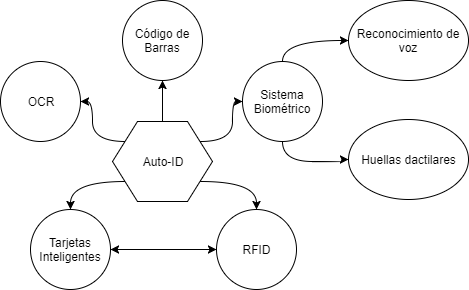
\includegraphics[scale=0.5]{tipos_rfid.png}
\centering
\caption{Tipos de Auto-ID}
\label{fig:tipos_rfid}
\end{figure}

La tecnología \textit{RFID} brinda información segura y permiten llevar un control eficiente del estado de los productos a muy bajo costo. El RFID nace como una evolución natural dedicada a identificar o realizar un seguimiento de personas, productos o animales. En comparación al código de barras, éste es capaz de almacenar más datos en memoria y permite la intercomunicación simultanea de varios \textit{tags}. Un sistema RFID está compuesto generalmente por un interrogador o lector (\textit{PCD - Proximity Coupling Device}) y uno o varios transponders, que generalmente toma la forma de tarjetas personales y/o tarjetas adhesivas (\textit{PICC - Proximity Integrated Circuit Card}). Cada transponder (\textit{tag}) cumple el rol de portador de información, tales como datos o identificación de un producto. Debido a su reducido tamaño y peso son dispositivos ideales para ser transportados por personas y animales, o para ser adheridos en algún producto.

Los transponders RFID se pueden clasificar en dos tipos debido a la de su alimentación: Activos o Pasivos. Los tags activos requieren energía adicional para alimentar el circuito, y los pasivos no requieren alimentación externa para su funcionamiento. 

Un ejemplo de los tags pasivos puede ser la tarjeta \textit{SUBE (Sistema Único de Boleto Electrónico)}. La SUBE es un sistema implementado en la República Argentina a partir del año 2011 que permite a cada usuario con su respectiva tarjeta inteligente, abonar los viajes en colectivos, subtes, trenes y los peajes adheridas a la Red SUBE. Éstas tarjetas cumplen con la norma ISO 14443-A que se describirán en la sección \ref{sec:iso}.



\subsection{Clasificación y estandarización de los sistemas RFID}

Existe una gran variedad de organizaciones que han determinado los estándares para la Identificación por Radio Frecuencia (RFID) según intereses, aplicaciones o simplemente por globalización. Entre las más destacadas encontramos la \textit{ISO (International Organization for Standardization)}, \textit{IEC (International Electrotechnical Commission)}, \textit{ASTM (American Society for Testing and Materials)} o \textit{EPCglobal (Asociación entre EAN International y GS1 Uniform Code Council)}.

También existen algunos sectores industriales que han establecido guías, ya sea para una mejor adaptación a sus realidades particulares, o bien porque no existían. Algunos ejemplos de estas industrias los encontramos en la \textit{FSTC (Financial Services Technology Consortium)}, el \textit{ICAR (International Committee for Animal Recording), CompTIA (Computer Technology Industry Association)}, la \textit{IATA (International Air Transport Association)}, \textit{EMV Contactless (Europay, Mastercard y Visa)}, organizaciones gubernamentales, etc.

\subsubsection{Regulación del espectro electromagnético}

Los distintos países han asignado diferentes zonas del espectro radioeléctrico para la RFID,  sin embargo, la mayoría de los países han acordado utilizar para los \textbf{sistemas de baja frecuencia (LF)} las zonas de 125 y 134,2 kHz del espectro, y la frecuencia de 13,56 MHz para los sistemas de \textbf{alta frecuencia (HF)}. Pero los \textbf{sistemas de ultra alta frecuencia (UHF)}, existen solo desde la segunda mitad de la década de los años 90 y los países no han acordado una sola zona del espectro para dicha banda, de manera que es mas complejo satisfacer óptimamente todos los requerimientos de los mercados existentes y/o potenciales.

En la Tabla \ref{table:rango_frec} se observa la diversidad de rangos del espectro UHF utilizados en diferentes países y regiones del mundo, mientras que en las bandas LF y HF se utilizan las mismas frecuencias.

\begin{table}[H]
\centering
\caption{Clasificación y rango de frecuencias}
\label{table:rango_frec}
\begin{tabular}{c|c|c|c}
\textbf{País o Región} & \textbf{LF}       & \textbf{HF} & \textbf{UHF}                                                                                \\ \hline
USA                    & 125 $-$ 134,2 kHz & 13,56 MHz   & 902 $-$ 928 MHz                                                                             \\
Europa                 & 125 $-$ 134,2 kHz & 13,56 MHz   & 865 $-$ 868 MHz                                                                             \\
Japón                  & 125 $-$ 134,2 kHz & 13,56 MHz   & 952 $-$ 954 MHz                                                                             \\
China                  & 125 $-$ 134,2 kHz & 13,56 MHz   & \begin{tabular}[c]{@{}c@{}}B1 = 840,5 $-$ 844,5 MHz\\ B2 = 920,5 $-$ 924,5 MHz\end{tabular} \\
Argentina              & 125 $-$ 134,2 kHz & 13,56 MHz   & 902 $-$ 928 MHz                                                                            
\end{tabular}
\end{table}

\subsubsection{Estándares establecidos}

Las familia de normas \textbf{ISO 18000} se han desarrollado para garantizar la interoperabilidad entre los sistemas RFID. Es el estándar que describe las diferentes tecnologías y/o frecuencias para la gestión a nivel de artículos. Las diferentes partes de este estándar describen la interface de comunicación vía aire de las distintas frecuencias para establecer los distintos comportamientos físicos.

Las distintas partes son:
\begin{itemize}
\item \textbf{Parte 1}: Arquitectura de referencia y definición de los parámetros estandarizados.
\item \textbf{Parte 2}: Parámetros establecidos para la interface de comunicación vía aire aplicados a los sistemas que funcionan a 135 KHz.
\item \textbf{Parte 3}: Parámetros establecidos para la interface de comunicación vía aire aplicados a los sistemas que funcionan a 13,56 MHz.
\item \textbf{Parte 4}: Parámetros establecidos para la interface de comunicación vía aire aplicados a los sistemas que funcionan a  2,45 GHz.
\item \textbf{Parte 5}: Parámetros establecidos para la interface de comunicación vía aire aplicados a los sistemas que funcionan a 5,8 GHz (fue retirada por falta de uso).
\item \textbf{Parte 6}: Parámetros establecidos para el interface de comunicación vía aire aplicados a los sistemas que funcionan entre 860 MHz y 960 MHz.
\item \textbf{Parte 7}: Parámetros establecidos para el interface de comunicación activo vía aire aplicados a los sistemas que funcionan a 433 MHz.
\end{itemize}

\subsubsection{Estándares LF}

\begin{itemize}
\item \textbf{ISO 14223} - Es el estándar que especifica la estructura del código de radiofrecuencia (RF) para transponders usados en animales. Esta norma es una extensión de los otros estándares \textbf{ISO 11784} e \textbf{ISO 11785}.
\item \textbf{ISO 11784} - Especifica la estructura del código de identificación
\item \textbf{ISO 11785} - Especifica la interface de comunicación vía aire aplicados a los sistemas que funcionan a 134,2 KHz, en la cual se definen y aprueban dos sistemas de intercambio de información: \textit{FDX-B (Full duplex)} y \textit{HDX (Half duplex)}.
\end{itemize}

\subsubsection{Estándares HF} 

\begin{itemize}
\item \textbf{ISO 14443} - Es el estándar basado en la frecuencia de 13,56 MHz \textit{(HF)} y es conocido como el estándar de tarjetas de proximidad o tarjetas con circuito integrado sin contacto.
\item \textbf{ISO 15692} - Protocolo de los datos usados en el intercambio de información en los sistemas RFID para la gestión de ítems, operando con el proceso de datos y la presentación en el tag RFID, así como el procesamiento inicial de los datos capturados desde transponder.
\item \textbf{ISO 15693} - Este estándar está basado también en la frecuencia de 13,56 MHz \textit{(HF)} y es conocido como el estándar para las tarjetas de vecindad \textit{(vicinity cards)}. La diferencia principal es la distancia de lectura/escritura que este estándar regula llegando a alcanzar 1,5 metros de distancia. Una de las claves de esta mayor distancia respecto a las tarjetas de proximidad (ISO 14443) es el campo magnético necesario para su activación, siendo de 0,15 a 5 A/m (1,5 a 7,5 A/m para la ISO 14443).
\item \textbf{ISO 18092} - Estándar que describe el intercambio de información sin contacto entre sistemas, conocido también como \textit{NFC (Near Field Communication – interface y protocolo NFCIP-1)}.
\item \textbf{ISO 21481} - Sistemas de intercambio de información y telecomunicaciones entre sistemas, \textit{Near Field Communications interface y protocolo – 2 (NFCIP-2)}.
\item \textbf{EMV Contactless} - Especificaciones para los sistemas de pago que define la arquitectura y requisitos generales, puntos de partida, especificaciones del kernel y el protocolo de comunicaciones contactless. Se basa en la \textbf{ISO 7816} y la \textbf{ISO 14443}.
\end{itemize}

\subsubsection{Estándares UHF}

\begin{itemize}
\item \textbf{ISO 18000-6} - Especifica los requisitos físicos y lógicos para un sistema de retrodispersión pasiva (passive-backscatter). El Lector recibe información de una etiqueta transmitiendo una señal de RF de onda continua (CW) a la etiqueta; la etiqueta responde modulando el coeficiente de reflexión de su antena, con lo cual retrodispersa una señal de información al Lector. 
\item \textbf{ISO 18000-61 – Type A} - El sistema es \textit{ITF (Interrogator-Talks-First)}, lo que significa que una etiqueta modula su coeficiente de reflexión de la antena con una señal de información solo después de ser dirigido por un Lector. Las etiquetas del tipo A utilizan la codificación \textit{PIE (Pulse-Interval Encoding)} en el enlace directo, y el algoritmo anti-colisión llamado \textit{ALOHA}.
\item \textbf{ISO 18000-62 – Type B} - El sistema es \textit{ITF} como las del tipo A, pero utiliza Codificación Manchester en el enlace directo, y como algoritmo anti-colisión \textit{binary-tree}.
\item \textbf{ISO 18000-63 – Type C} - El sistema es \textit{ITF} y utiliza Codificación \textit{PIE} como las de tipo A, pero como algoritmo anti-colisión utiliza \textit{random slotted}.
\item \textbf{ISO 18000-64 – Type D} - El sistema es \textit{TOTAL (Tag Only Talks After Listening)}, lo que significa que una etiqueta modula su coeficiente de reflexión de antena con una señal de información al ingresar al campo de un Lector, después de escuchar por primera vez la modulación del Lector para determinar si el sistema es o no ITF. La codificación de las etiquetas del tipo D es por posición de pulso \textit{(Pulse Position Encoding)} o \textit{Miller M = 2}.
\item \textbf{EPC UHF Class1 Gen2} – Las etiquetas \textit{RFID EPC} Clase 1 Gen-2 se utilizan para identificar un artículo en la cadena de suministro a nivel mundial. "Clase 1" se refiere a la funcionalidad de la etiqueta, mientras que "Gen-2" se refiere a los estándares físicos y lógicos de la etiqueta y el sistema abarcador. Estos estándares son mantenidos por \textit{EPCglobal}. 
\end{itemize}

\subsection{Norma ISO/IEC 14443} \label{sec:iso}

ISO/IEC 14443 es un estándar internacional relacionado con las tarjetas de identificación por radiofrecuencia (RFID), en especial para las tarjetas de proximidad, gestionado conjuntamente por la Organización Internacional de Normalización (ISO) y Comisión Electrónica Internacional (IEC).

Ésta norma consiste en 4 partes:
\begin{itemize}
	\item \textbf{Parte 1:} Especifica las características físicas.
	\item \textbf{Parte 2:} Especifica la potencia RF, los distintos tipos de modulación y la interfaz con el \textit{core} digital.
	\item \textbf{Parte 3:} Especifica la inicialización y anticolisión entre los chips.
	\item \textbf{Parte 4:} Especifica el protocolo de transmisión de datos. 
\end{itemize}

\subsection{Norma ISO/IEC 14443 Parte 1: Características físicas}

Ésta primera parte, al comienzo define los símbolos y abreviaciones que se utilizará a lo largo de la norma. Entre ellas, las más relevantes son:

\begin{itemize}
	\item \textbf{Proximity Integrated Circuit Card (PICC)}: Es el dispositivo portador de la información, generalmente tiene forma de tarjeta \textit{(tag)}.
	\item \textbf{Proximity Coupling Device (PCD)}: Es el dispositivo que produce el campo magnético y comunica con el PICC a través de acoplamiento inductivo.
\end{itemize}

En cuanto a características físicas, se define el tamaño y forma que tiene que tener la antena (86 x 54 x 3) mm, ya que la interfaz de radiofrecuencia y los bancos de prueba, que están definidos en la norma ISO/IEC 10373-6, son para una antena del tamaño de una tarjeta ID-1. El estándar ISO/IEC 7810 define el tamaño de éste tipo de tarjetas.

También se incluye información acerca de la radiación ultravioleta, rayos X, y temperaturas de operación para la PICC.

\subsection{Norma ISO/IEC 14443 Parte 2: Alimentación e interferencia de la señal de RF}
\label{sec:Norma14443-2}
En ésta segunda parte se especificará la naturaleza y las características de los campos que deben proveerse para alimentar y poder establecer una comunicación bidireccional entre el dispositivo de acoplamiento (\textit{PCD}) y las tarjetas de proximidad (\textit{PICC}). Como introducción sólo se presentará la interfaz de comunicación tipo A \cite{nfc_spec}.

\subsubsection{Términos y definiciones} 
\begin{itemize}
\item \textbf{Duración del bit:} Tiempo durante el cual un estado lógico es definido, al finalizar este un nuevo bit comienza.
\item \textbf{Modulación binaria por desplazamiento de fase:} Modulación de los estados con un desplazamiento de 180°, como resultado se tienen dos estados posibles.
\item \textbf{Índice de modulación:} Definido como $\frac{a-b}{a+b}$ donde a y b representan la máxima y mínima amplitud de la señal respectivamente.
\item \textbf{NRZ-L:} Método de codificación binaria mediante el cual un estado lógico posee la duración del bit y es representado por uno de dos estado físico definidos en el medio de comunicación.
\item \textbf{Subportadora:} La señal de RF producida por la modulación de una portadora de frecuencia fc con una señal de frecuencia fs.
\end{itemize}

\subsubsection{Diálogo inicial de las tarjetas de proximidad}

El diálogo inicial entre el PCD y el PICC debe respetar las siguientes operaciones en forma consecutiva.
Activar el PICC sometiéndolo al campo de RF generado por el PCD.
\begin{itemize}
\item El PICC entra al campo RF.
\item El PICC espera al comando del PCD.
\item El PCD transmite un comando.
\item El PICC transmite la respuesta.
\end{itemize}

Estas operaciones usan la energía de RF y la interfaz especificada en las siguientes cláusulas.

\begin{itemize}
\item \textbf{Transferencia de energía:} El PCD deberá producir un campo energizante de RF que acople el PICC para transferir la energía y el cual estará modulado para la comunicación.
\item \textbf{Frecuencia:} La frecuencia de la portadora (fc) deberá ser de 13.56MHz +- 7KHz.
\item \textbf{Campo operativo:} El campo mínimo sin modulación deberá ser de 1.5A/m (RMS) y el máximo de 7.5 A/m (RMS). Tanto el PCD como el PICC deberá operar entre estos rangos. El método para testear el campo generado por el PCD está definido en la ISO/IEC 10373.
\end{itemize}

\subsubsection{Interferencia de la señal}

Las dos interfaces de comunicación (tipo A y tipo B) están descriptas a continuación.

El PCD deberá alternar entre los métodos de modulación antes de la detección de la presencia de un PICC tipo A o tipo B. Sólo una interfaz de comunicación podrá estar activada durante una sesión de comunicación hasta la desactivación del PCD o la sustracción del PICC. La o las sesiones subsecuentes podrán proceder usando cualquier método de modulación. Los dos distintos tipos de interfaces se puede observar en la figura \ref{fig:tipos_iso}.

\begin{figure}[H]
\centering
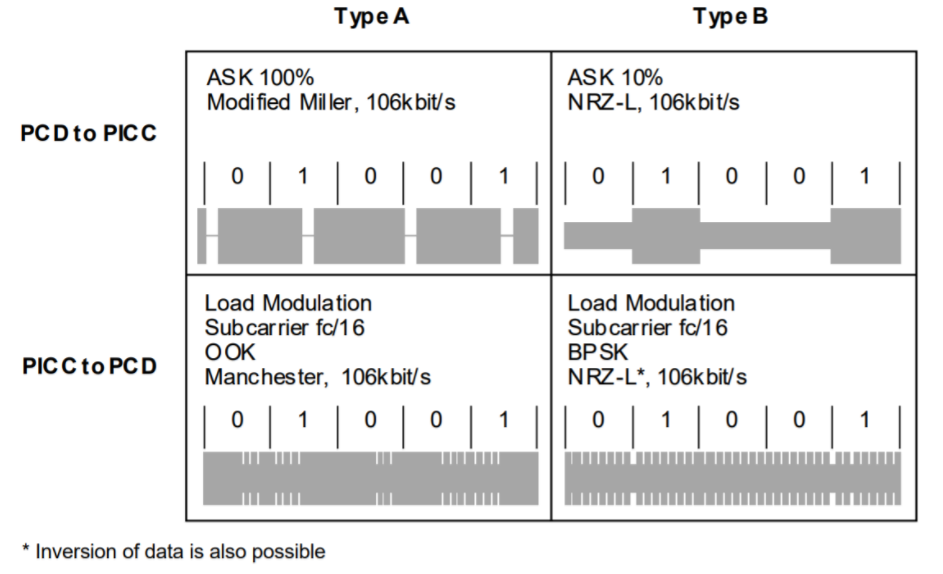
\includegraphics[width=0.9\linewidth]{otros/tipos_iso.png}
\caption{Tipos de inteface ISO/IEC 14443}
\label{fig:tipos_iso}
\end{figure}

\subsubsection{Interfaz de comunicación tipo “A”}

\begin{enumerate}
\item Comunicación PCD a PICC
\begin{itemize}
\item \textbf{Velocidad de transmisión:} durante la inicialización y anticolisión la velocidad de transmisión deberá ser fc/128.
\item \textbf{Modulación:} La comunicación entre el PCD y el PICC se lleva a cabo empleando el principio de modulación ASK 100\% del campo RF para crear la “pausa” como se muestra en la figura \ref{fig:demod_tipoa}.

\begin{figure}[H]
\centering
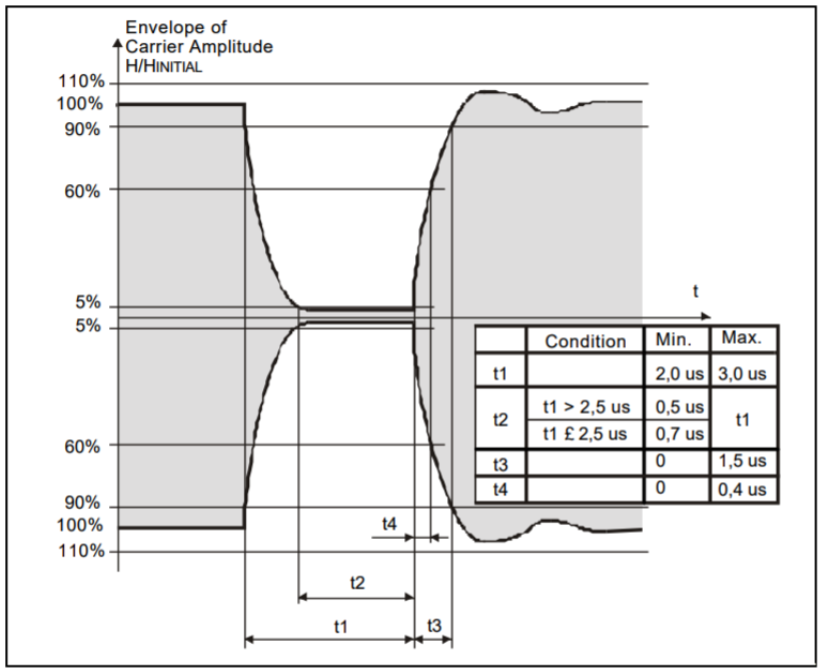
\includegraphics[width=0.7\linewidth]{otros/demod_tipoa.png}
\caption{Modulación PCD a PICC}
\label{fig:demod_tipoa}
\end{figure}

La envolvente del campo del PCD deberá decrementar monótonamente a menos del 5\% de su valor inicial (Hinicial) y permanecer de esta manera por un tiempo mayor a “t2”.

Si la envolvente del campo del PCD no decrementa monótonamente, el tiempo entre un máximo local y el tiempo del paso del mismo valor antes del máximo local no deberá exceder  los 0.5us. Esto solo aplicará si el máximo local es mayor al 5\% del H inicial.

El sobrepaso deberá permanecer entre el 90\% y el 110\% del H inicial.

El PICC deberá detectar el “Fin de pausa” (End of Pause) luego de que el campo exceda el 5\% del H inicial y antes de que supere el 60\% del mismo.

En la figura \ref{fig:pausa_tipoa} se procede a mostrar la definición del “Fin de Pausa” (EoP).

\begin{figure}[H]
\centering
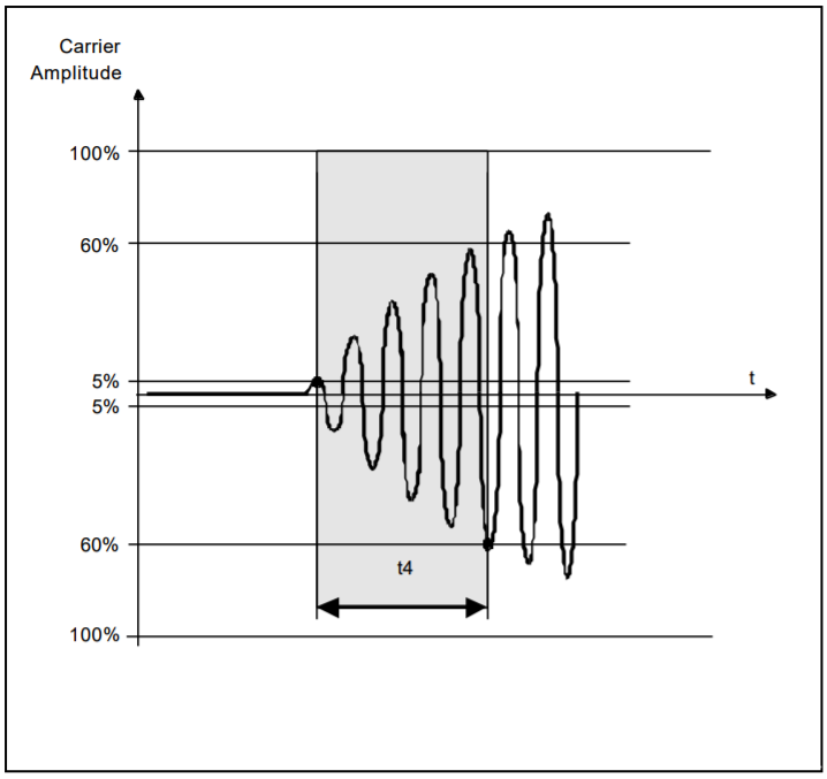
\includegraphics[width=0.7\linewidth]{otros/pausa_tipoa.png}
\caption{Fin de la pausa - ISO/IEC 14443A}
\label{fig:pausa_tipoa}
\end{figure}

\item \textbf{Representación de los bits y codificación:} Las secuencias están definidas en la tabla \ref{fig:code_tipoa} y la codificación en la tabla \ref{fig:dem_cod_tipoa}.

\begin{figure}[H]
\centering
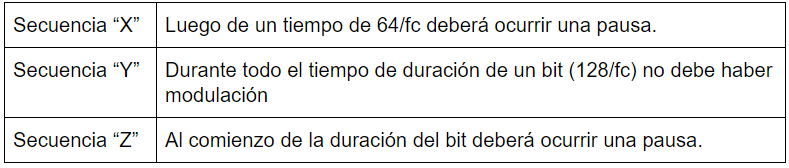
\includegraphics[width=0.9\linewidth]{otros/secuencia_tipoa.png}
\caption{Secuencia PCD a PICC}
\label{fig:code_tipoa}
\end{figure}

\begin{figure}[H]
\centering
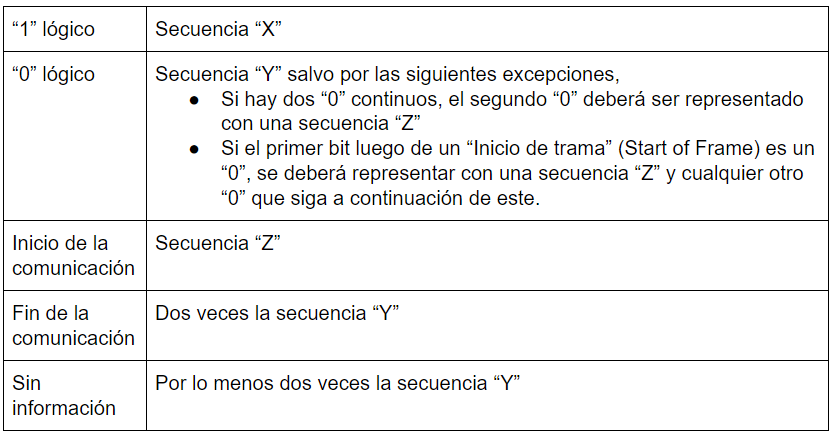
\includegraphics[width=0.9\linewidth]{otros/dem_codigo_tipoa.png}
\caption{Codificación PCD a PICC}
\label{fig:dem_cod_tipoa}
\end{figure}


\end{itemize}

\item Comunicación PICC a PCD

\begin{itemize}
\item \textbf{Velocidad de la información:} Al igual que la comunicación del PCD al PICC, la velocidad durante la inicialización y la anticolisión deberá ser de fc/128 (106 kbit/s).
\item \textbf{Carga de la modulación:} El PICC debera ser capaz de comunicarse hacía el PCD a través del acoplamiento inductivo en donde la frecuencia de la portadora será empleada para generar una subportadora de frecuencia fs. Esta subportadora deberá ser generada empleando una carga en el PICC. La amplitud de la modulación deberá ser por lo menos de 30/H mV, en donde H será el valor RMS de la fuerza del campo magnético en A/m.
\item \textbf{Subportadora:} La frecuencia fs debe ser de fc/16 (847kHz). Consecuentemente con esto, durante la inicialización y la anticolisión, la duración de un bit será equivalente a 8 periodos de la subportadora.
\item \textbf{Modulación de la subportadora:} Cada bit comienza su periodo con una fase definida en relación con la subportadora. El periodo del mismo comienza con el estado cargado de la subportadora. Esta deberá ser modulada usando modulacion on/off con las secuencias definidas en la tabla \ref{fig:mod_cod_tipoa}.

\begin{figure}[H]
\centering
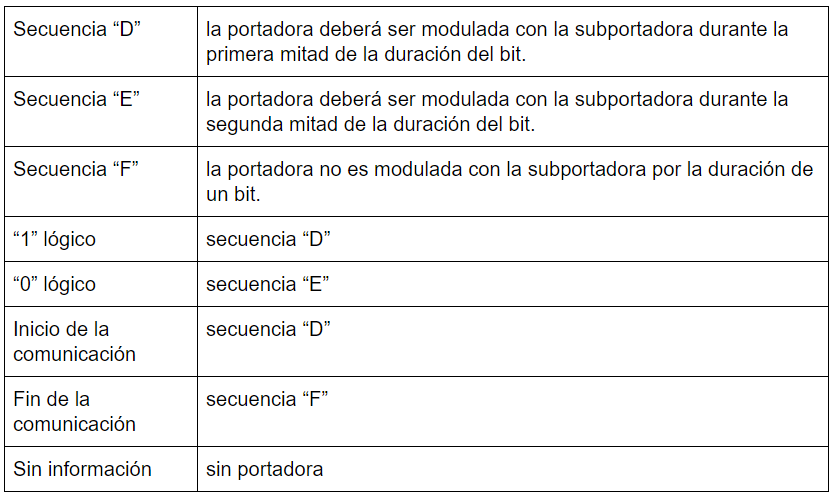
\includegraphics[width=0.9\linewidth]{otros/mod_codigo_tipoa.png}
\caption{Codificación PICC a PCD}
\label{fig:mod_cod_tipoa}
\end{figure}

\end{itemize}


\end{enumerate}

\subsection{Norma ISO/IEC 14443 Parte 3: Inicialización y anticolisión}
\label{sec:Norma14443-3}
%%%%%%%%%%%%%%%%%%%% Document code starts here %%%%%%%%%%%%%%%%%%%%
\subsubsection{Alcance}
Esta parte de la norma describe\par

\begin{itemize}
	\item Sondeo para PICC’s que ingresan al campo de un PCD.\par

	\item El formato de los bytes, tramas y la sincronización empleada durante la fase inicial de la comunicación entre el PCD y el PICC.\par

	\item Contenido del comando inicial REQ y ATQ.\par

	\item Otros parametros requeridos para la inicialización de la comunicación entre los dispositivos.
\end{itemize}\par

\subsubsection{Normativa de referencia}
Las siguientes normas realizan un aporte para constituir un estándar internacional.\par

\begin{itemize}
	\item ISO/IEC 3309: 1993 Intercambio de información entre sistemas de telecomunicaciones. (High Level Data Link Control)\par

	\item ISO/IEC 7816: 1997 Circuitos integrados en tarjetas con contactos.\par

	\item ISO/IEC 14443/2: Circuitos integrados en tarjetas sin contactos - Tarjetas de proximidad.\par

	\item ITU-T Recomendations V.41
\end{itemize}\par

\subsubsection{Términos y definiciones}
Para los propositos de este estándar internacional los términos y definiciones dados en ISO/IEC 14443-2, ISO/IEC 7816-3 y los siguientes aplican.\par

\paragraph{Loop anti-colisión}
Algoritmo empleado para preparar al PCD para dialogar entre una o más PICC’s dentro de su campo energizante.\par


\vspace{\baselineskip}
\paragraph{Protocolo detección de colisión de bits}
Método de anticolisión empleando detección de colisión a nivel de los bits entre tramas. Una colisión ocurre cuando al menos dos PICC’s transmiten patrones complementarios de bits (ver ISO/IEC 14443-2 sección 8.4.2) hacia el PCD. En este caso los patrones de bits son unidos y la portadora es modulada con la subportadora durante toda la duración del bit.\par

El PCD detecta la colisión de bits y reconoce todos los PICC’s en orden de cascada\par


\vspace{\baselineskip}
\paragraph{Byte}
Un byte consta de 8 bits de datos designados b1 a b8, comenzando por el bit más significativo (MSB, b8) hacia el bit menos significativo (LSB, b1).\par


\vspace{\baselineskip}
\paragraph{Colisión}
La transmisión de dos PICC’s en el mismo campo energizante de un PCD y durante el mismo periodo de tiempo, tanto como para que el PCD no logre distinguir el PICC originario de la información.\par


\vspace{\baselineskip}
\paragraph{Unidad Elemental de Tiempo (ETU)}
Para esta parte de la ISO/IEC 14443, un ETU esta definido como\par

\paragraph{Trama (Frame)}
Una trama es una serie de bits de información y, opcionalmente, bits para detección de errores, con delimitadores de trama al inicio y al final de la misma.\par

\paragraph{Capa superior}
Perteneciendo a la aplicación o a capas superiores del protocolo, esto no será descripto en este apartado.\par

\paragraph{Protocolo de intervalo temporal}
Método en donde el PCD establece los canales lógicos con uno o más PICC’s, en el cual se realiza la asignación de los intervalos temporales para la respuesta del PICC.\par

\paragraph{Identificador Único (UID)}
Es un número necesario para el algoritmo de anti-colisión del $``$Tipo A$"$ .\par

\subsubsection{Simbolos (y terminos abreviados)}
Para esta parte de la norma, las abreviaturias utilizadas son:\par

\begin{itemize}
	\item AFI Application Familly Identifie.\par

	\item APa Anticolisión Prefijo a, usado en ATQB\par

	\item APc Anticolisión Prefijo c, usado en Attribute\par

	\item APf Anticolisión Prefijo f, usado en REQB\par

	\item APn Anticolisión Prefijo n, usado en el comando Slot-MARKER\par

	\item ATA Respuesta a ATTRIB\par

	\item ATQ Respuesta a REQUEST\par

	\item ATQA Respuesta a REQUEST del Tipo A\par

	\item ATQB Respuesta a REQUEST del Tipo B\par

	\item ATTRIB Comando de selección del PICC\par

	\item BCC UID CLn checkbyte, calculado como una or exclusivede los 4 bytes anteriores\par

	\item CLn Nivel de cascada\par

	\item CT Tag de cascada, ‘88’\par

	\item CRC\_A Código del ciclo de chequeo redundante de errores definido en 6.1.10\par

	\item CRC\_B Ciclo de chequeo redundante de errores definido en 7.2\par

	\item DESEL Comando para anular la selección\par

	\item E Fin de la comunicación del Tipo A\par

	\item EGT Tiempo de guarda extra (Extra Guard Time)\par

	\item EOF Fin de la trama (End Of Frame), Tipo B\par

	\item ETU Unidad de tiempo elemental, duración de un bit de la transmisión.\par

	\item FGT\ Tiempo de guarda de  la trama (Frame Guard Time)\par

	\item Fc Frecuencia de portadora (13,56 MHz)\par

	\item Fs Frecuencia de la subportadora\par

	\item ID Número de identificación\par

	\item INF Campo de información perteneciente a la capa superior\par

	\item LSB Bit menos significativo (Least Significant Bit)\par

	\item MSB Bit más significativo (Most Significant Bit)\par

	\item N Cantidad de espacios para la anticolisión.\par

	\item NAD Dirección del nodo (Node ADdress)\par

	\item NVB Número de bits validos (Number of Valid Bits)\par

	\item P Bit de paridad impar (Odd parity bit)\par

	\item PARAM Parámetro\par

	\item PCD Dispositivo de acoplamiento de proximidad (Proximity Coupling Device)\par

	\item PICC Tarjeta de proximidad\par

	\item PUPI Identificador Pseudo-Único del PICC\par

	\item REQA Comando de solicitud (Request Command), Tipo A\par

	\item REQB Comando de solicitud (Request Command), Tipo B\par

	\item S Inicio de la comunicación, Tipo A\par

	\item SAK Reconocimiento de SELECT\par

	\item SEL Comando SELECT\par

	\item SOF Inicio de trama $\ast$ Start Of Frame), Tipo B\par

	\item UID Identificador Único (Unique IDentification)\par

	\item UIDn Cantidad de bytes del UID
\end{itemize}\par

\subsubsection{Sondeo}
Cuando un PICC se expone a un campo operativo no modulado (ver ISO / IEC 14443-2), debe poder aceptar una solicitud dentro de los 5 ms.\par

Por ejemplo, \par

Cuando un PICC tipo A recibe cualquier comando de tipo B, debe poder aceptar un REQA dentro de los 5 ms.\par

Cuando un PICC tipo B recibe un comando de tipo A, debe poder aceptar un REQB dentro de los 5 ms.\par

Con el fin de detectar los PICCs que entran en su campo energizante, un PCD envía comandos de Solicitud repetidos y busca un ATQ. Los comandos de solicitud usarán REQA y REQB descritos en este documento en cualquier secuencia y además podrán usar otros codificación (es) descrita (s) en el Anexo C. Este proceso se denomina "Sondeo".\par

\subsubsection{Tipo A - Inicialización y anticolisión}
Esta sección describe el protocolo de detección de colisiones de bits aplicable para los PICC de tipo A.\par

\paragraph{Byte, formato de trama y comando y tiempo.}
Esta sección define los formatos del byte de la trama del comando y el tiempo utilizado durante la inicialización de la comunicación y anticolisión. Para la representación y codificación de bits, consulte ISO / IEC 14443-2.\par

\paragraph{Tiempo de retardo de trama}
El tiempo de retardo de trama (FDT) se define como el tiempo entre dos tramas transmitidas en direcciones opuestas.\par

\paragraph{Tiempo de protección de trama}
El tiempo de protección de trama (FGT) se define como el tiempo de retardo de trama mínimo.\par

\paragraph{Tiempo de retardo de trama PCD a PICC}
Este es el tiempo entre el final de la última pausa transmitida por el PCD y el primer borde de modulación dentro del bit de inicio transmitido por el PICC, deberá respetar el tiempo definido en la figura 6.1, donde n es un valor entero.\par


\vspace{\baselineskip}


%%%%%%%%%%%%%%%%%%%% Figure/Image No: 1 starts here %%%%%%%%%%%%%%%%%%%%

\begin{figure}[H]
	\begin{center}
		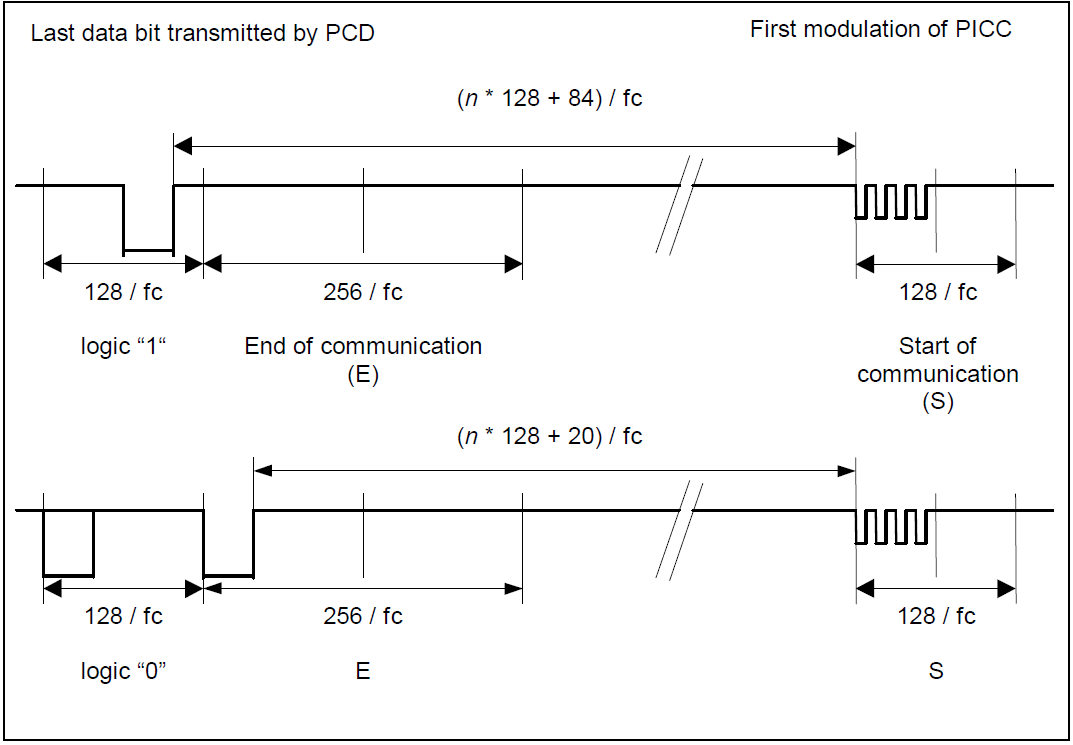
\includegraphics[width=6.1in,height=4.22in]{Norma_ISO/14443-3/media//image9.png}
        \end{center}
\end{figure}


%%%%%%%%%%%%%%%%%%%% Figure/Image No: 1 Ends here %%%%%%%%%%%%%%%%%%%%

\par
\begin{center}
Figura 3.7.6.1 - Demora temporal de trama PCD a PICC.
\end{center}
\par


\paragraph{Tiempo de retardo trama PICC a PCD}
Este es el tiempo transcurrido entre la última modulación transmitida por el PICC y la primera pausa transmitida por el PCD y deberá ser al menos 1172 / fc.\par

\paragraph{Tiempo de guardia de solicitud}
El Tiempo de guardia de solicitud se define como el tiempo mínimo entre los bits de inicio de dos comandos REQUEST consecutivos. Eso tiene el valor 7000 / fc.\par

\paragraph{Formatos de trama}
Los siguientes tipos de tramas se definen para el protocolo de detección de colisiones de bits.\par

\paragraph{Tramas REQA y WAKE-UP}
Las tramas de solicitud (REQA) y activación (WAKE-UP) se utilizan para iniciar la comunicación y consisten en, en el siguiente orden:\par

\begin{itemize}
	\item Inicio de comunicación\par

	\item 7 bits de datos transmitidos LSB primero. (El contenido de los datos es '26' para un REQA estándar y '52' para una solicitud de WAKE-UP).\par

	\item Fin de la comunicación
\end{itemize}\par

No se agrega bit de paridad.\par

%%%%%%%%%%%%%%%%%%%% Figure/Image No: 2 starts here %%%%%%%%%%%%%%%%%%%%
\begin{figure}[H]
	\begin{center}
		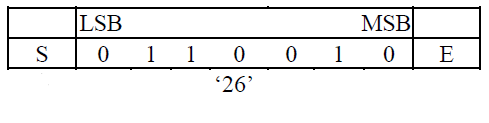
\includegraphics[width=3.76in,height=0.95in]{Norma_ISO/14443-3/media/image6.png}
        \end{center}
\end{figure}
%%%%%%%%%%%%%%%%%%%% Figure/Image No: 2 Ends here %%%%%%%%%%%%%%%%%%%%

\par
\begin{center}
Figura 3.7.6.2 -Tramas REQA y WAKE-UP.
\end{center}
\par

\par
\paragraph{Trama estándar}
Las tramas estándar se utilizan para el intercambio de datos y consisten en,\par

\begin{itemize}
	\item Inicio de comunicación\par

	\item N $\ast$  (8 bits de datos + bit de paridad impar). El LSB de cada byte de datos se transmite primero. Cada byte de datos es seguido por un bit de paridad impar.\par

	\item Fin de la comunicación
\end{itemize}\par

\paragraph{Marco de anticolisión orientado a bits}
Se detecta una colisión cuando al menos dos PICC transmiten patrones de bits diferentes a la PCD. En este caso, la portadora se modula con la subportadora durante toda la duración del bit para al menos un bit.\par

Las tramas de anticolisión orientadas a bits solo se utilizan durante los ciclos anticolisión de tramas de bits y son, de hecho, tramas estándar con una longitud de 7 bytes de datos, divididos en dos partes: parte 1 para transmisión de PCD a PICC y parte 2 para transmisión desde PICC a PCD.\par

Para la duración de la parte 1 y parte 2, se aplicarán las siguientes reglas:\par

Regla 1: La suma de los bits de datos será 56\par

Regla 2: la longitud mínima de la parte 1 será de 16 bits de datos\par

Regla 3: la longitud máxima de la parte 1 será de 55 bits de datos\par

En consecuencia, la longitud mínima de la parte 2 será de 1 bit de datos y la longitud máxima será de 40 bits de datos.\par

Como la división puede ocurrir en cualquier posición de bit dentro de un byte de datos, se definen dos casos:\par

Caso FULL BYTE: división después de un byte de datos completo. Se agrega un bit de paridad después del último bit de datos de la parte 1.\par

Caso SPLIT BYTE: división dentro de un byte de datos. No se agrega ningún bit de paridad después del último bit de datos de part1.\par

\paragraph{CRC\_A}
El proceso de codificación y verificación CRC\_A se define en la recomendación UIT-T V.41, párrafo 2. El polinomio generador utilizado para generar los bits de verificación es x $ \string^ $  16 + x $ \string^ $  12 + x $ \string^ $  5 + 1. El valor inicial será ' 6363 '. El CRC\_A se adjuntará a los bytes de datos y se transmitirá a través de tramas estándar.\par

\paragraph{Estados del PICC.}
Las siguientes secciones proporcionan descripciones de los estados para un PICC de tipo A específico del protocolo de detección de colisiones de bits.\par



%%%%%%%%%%%%%%%%%%%% Figure/Image No: 3 starts here %%%%%%%%%%%%%%%%%%%%

\begin{figure}[H]
	\begin{center}
		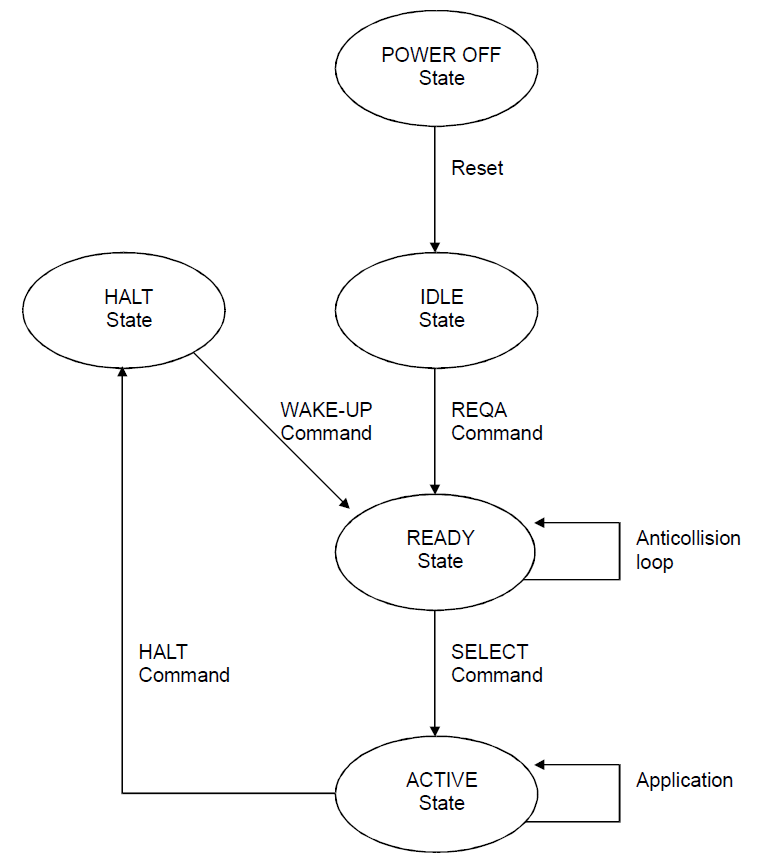
\includegraphics[width=6.27in,height=7.01in]{Norma_ISO/14443-3/media/image7.png}
        \end{center}
\end{figure}


%%%%%%%%%%%%%%%%%%%% Figure/Image No: 3 Ends here %%%%%%%%%%%%%%%%%%%%

\par

\par
\begin{center}
Figura 3.7.6.3 - Diagrama de estados PICC Tipo $``$A$"$ 
\end{center}
\par

\paragraph{Estado OFF}
En el estado de OFF, el PICC no recibe energía debido a la falta de energía del portador y no debe emitir subportadora.\par

\paragraph{Estado IDLE}
Después de que el campo haya estado activo durante un retraso máximo definido en la cláusula 5, el PICC ingresará en su estado IDLE. En este estado, el PICC está encendido, y es capaz de demodular y reconocer los comandos válidos de REQA y WAKE-UP del PCD.\par

\paragraph{Estado READY}
Este estado se ingresa tan pronto como se recibe y sale un mensaje REQA o WAKE-UP válido cuando el PICC está seleccionado con su UID. En este estado, se puede aplicar la anticolisión de la trama de bits u otro método anticolisión opcional. Los niveles de cascada se manejan dentro de este estado para obtener todo el UID CLn.\par

\paragraph{Estado ACTIVE}
Este estado se ingresa seleccionando el PICC con su UID completo.\par

\paragraph{Estado HALT}
Este estado se ingresa mediante el comando HALT definido en 3.7.6.3.4 o mediante un comando específico de la aplicación no definido en esta parte de ISO / IEC 14443. En este estado, un PICC responderá solo a un comando de WAKE-UP, que transita el PICC a su estado READY.\par

\paragraph{Conjunto de comandos}
Los comandos utilizados por el PCD para gestionar la comunicación con varios PICC son:\par

\begin{itemize}
	\item REQA\par

	\item WAKE-UP\par

	\item ANTICOLLISION\par

	\item SELECT\par

	\item HALT
\end{itemize}\par

Los comandos usan los formatos de byte y marco descriptos anteriormente.\par

\paragraph{Comando REQA}
El comando REQA es enviado por el PCD para sondear el campo de los PICC de tipo A.\par

\paragraph{Comando WAKE-UP}
El PCD envía el comando WAKE-UP para poner los PICC que han ingresado al estado HALT de nuevo en el estado READY. Luego, participarán en nuevos procedimientos de anticolisión y selección.\par

\paragraph{Comandos ANTICOLLISION y SELECT}
Estos comandos se usan durante un ciclo anticolisión. Los comandos ANTICOLLISION y SELECT constan de:\par

\begin{itemize}
	\item Seleccionar código SEL (1 byte)\par

	\item Número de bits válidos NVB (1 byte)\par

	\item De 0 a 40 bits de datos de UID CLn según el valor de NVB
\end{itemize}\par

SEL especifica el nivel de cascada CLn.\par

NVB especifica el número de bits válidos de UID CLn transmitidos por el PCD.\par

\paragraph{Comando HALT}
El comando HALT consta de cuatro bytes y se transmitirá utilizando la trama estándar.\par



%%%%%%%%%%%%%%%%%%%% Figure/Image No: 4 starts here %%%%%%%%%%%%%%%%%%%%

\begin{figure}[H]
	\begin{center}
		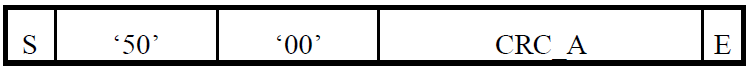
\includegraphics[width=5.47in,height=0.51in]{Norma_ISO/14443-3/media/image10.png}
        \end{center}
\end{figure}


%%%%%%%%%%%%%%%%%%%% Figure/Image No: 4 Ends here %%%%%%%%%%%%%%%%%%%%

\par
\begin{center}
Figura 3.7.6.4 - Trama del comando HALT.
\end{center}
\par

Si el PICC responde con cualquier modulación durante un período de 1 ms después del final de la trama HALT, esta respuesta se interpretará como "no reconocido".\par

\paragraph{Secuencia SELECT}
El propósito de esta secuencia es el de obtener el UID de un PICC y seleccionar a este PICC para una futura comunicación.\par

\paragraph{ATQA - Respuesta al comando REQA}
Después de que el PCD transmite el comando REQA, todos los PICC responden de forma síncrona con su respuesta (ATQA), que codifica el tipo anticolisión aplicable en dos bytes de datos.\par

Si hay múltiples respuestas PICC, pueden producirse colisiones. El PCD decodificará una colisión dentro de ATQA. Esto da como resultado un OR lógico de todos los ATQA.\par

\paragraph{Anticolisión y selección}
\paragraph{Bucle anticolisión dentro de cada nivel de cascada}
El siguiente algoritmo se aplicará al ciclo anticolisión:\par

\begin{itemize}
	\item Paso 1: El PCD asigna SEL con el código para el tipo de anticolisión seleccionado y el nivel de cascada.\par

	\item Paso 2: El PCD asigna NVB con el valor de '20'.\par

	\item Paso 3: El PCD transmite SEL y NVB.\par

	\item Paso 4: Todos los PICC en el campo responderán con su UID CLn completa.\par

	\item Paso 5: Suponiendo que los PICC en el campo tengan números de serie únicos, entonces, si responde más de un PICC, se produce una colisión. Si no ocurre una colisión, se omiten los pasos 6 a 10.\par

	\item Paso 6: El PCD reconocerá la posición de la primera colisión.\par

	\item Paso 7: El PCD asigna NVB con un valor que especifica el número de bits válidos de UID CLn. Los bits válidos serán parte del UID CLn que se recibió antes de que ocurriera una colisión añadida por un (0) by (1) b, decidido por el PCD. Una implementación típica agrega a (1) b.\par

	\item Paso 8: El PCD transmite SEL y NVB, seguidos de los bits válidos.\par

	\item Paso 9: Solo los PICC cuya parte de UID CLn es igual a los bits válidos transmitidos por el PCD transmitirán sus bits restantes del UID CLn.\par

	\item Paso 10: Si ocurren más colisiones, se repiten los pasos 6 a 9. La cantidad máxima de bucles será 32.\par

	\item Paso 11: Si no hay más colisiones, la PCD asigna NVB con el valor de '70'.\par

	\item Paso 12: El PCD transmite SEL y NVB, seguidos de los 40 bits de UID CLn, seguidos por CRC\_A suma de comprobación.\par

	\item Paso 13: El PICC que UID CLn coincide con los 40 bits responde con su SAK.\par

	\item Paso 14: Si el UID está completo, el PICC transmitirá SAK con un bit en cascada despejado y el tránsito desde el estado LISTO al estado ACTIVO.\par

	\item Paso 15: El PCD verificará si el bit en cascada de SAK está configurado para decidir si seguirán ciclos de anticolisión adicionales con un nivel de cascada incrementado.
\end{itemize}\par

Si el UID de un PICC es conocido, el PCD puede omitir el paso 2 al paso 10 para seleccionar este PICC sin realizar el ciclo anticolisión.\par

\paragraph{Código de SEL}
Longitud: 1 byte\par

Valores posibles: '93', '95', '97'.\par

\paragraph{Código de NVB (número de bits válidos)}
Longitud: 1 byte\par

Los 4 bits superiores se llaman por cuenta y especifican el número de todos los bits de datos válidos divididos entre 8, incluidos SEL y NVB transmitidos por el PCD. En consecuencia, el valor mínimo de bytecount es 2 y el valor máximo es 7.\par

Los 4 bits más bajos se denominan bitcount y especifican el número de todos los bits de datos válidos módulo 8 transmitidos por el PCD.\par

\paragraph{Código de SAK}
SAK es transmitido por el PICC cuando NVB ha especificado 40 bits de datos válidos y cuando todos estos bits de datos coinciden con UID CLn.\par

SAK se transmite a través la trama estándar, seguido de CRC\_A.\par

Si el UID no está completo, el PICC permanecerá en estado READY y el PCD iniciará un nuevo ciclo de anticolisión con un nivel de cascada incrementado.\par

Si el UID está completo, el PICC transmitirá SAK con el bit de cascada despejado y el tránsito del estado READY al estado ACTIVE. El PICC configurará el bit b6 de SAK cuando haya información adicional disponible.\par

La definición de la información adicional no está sujeta a esta parte del estándar y se definirá en ISO / IEC 14443-4.\par

\paragraph{Contenido de UID y niveles de cascada}
El UID consta de 4, 7 o 10 bytes UID. En consecuencia, el PICC manejará hasta 3 niveles de cascada para obtener todos los bytes de UID.\par

Dentro de cada nivel de cascada, una parte del UID que consta de 5 bytes de datos se transmitirá a la PCD. De acuerdo con la nivel de cascada máximo, se definen tres tipos de tamaño de UID. Este tamaño de UID debe ser consistente con la tabla 6.4.\par



%%%%%%%%%%%%%%%%%%%% Figure/Image No: 5 starts here %%%%%%%%%%%%%%%%%%%%

\begin{figure}[H]
	\begin{center}
		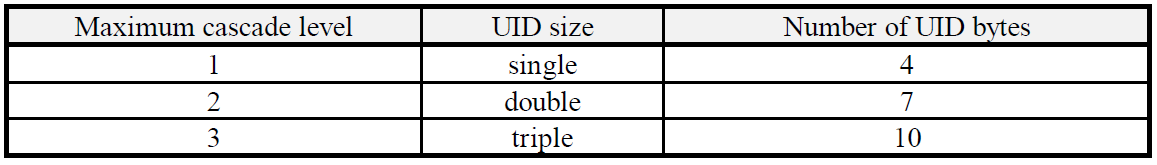
\includegraphics[width=6.27in,height=0.89in]{Norma_ISO/14443-3/media/image8.png}
        \end{center}
\end{figure}


%%%%%%%%%%%%%%%%%%%% Figure/Image No: 5 Ends here %%%%%%%%%%%%%%%%%%%%

\par
\begin{center}
Figura 3.7.6.4 - Tamaños de los UID.
\end{center}
\par

\subsection{Norma ISO/IEC 14443 Parte 4: Protocolo de transmisión}
\label{sec:Norma14443-4}
%%%%%%%%%%%%%%%%%%%% Document code starts here %%%%%%%%%%%%%%%%%%%%
\subsubsection{Alcance}
Esta parte de ISO / IEC 14443 especifica un protocolo de transmisión de bloques semidúplex que presenta las necesidades especiales de un entorno sin contacto y define la secuencia de activación y desactivación del protocolo.\par

Esta parte de ISO / IEC 14443 se utilizará junto con otras partes de ISO / IEC 14443 y se aplica a las tarjetas de proximidad de tipo A y tipo B.\par

\subsubsection{Referencias normativas}
Las siguientes normas contienen disposiciones que, a través de la referencia en este texto, constituyen disposiciones de esta parte de ISO / IEC 14443. En el momento de la publicación, las ediciones indicadas eran válidas. Todos los estándares están sujetos a revisión,\par

y se alienta a las partes de los acuerdos basados ​​en esta parte de ISO / IEC 14443 a investigar la posibilidad de aplicar las normas Internacionales válidas más recientes.\par

ISO / IEC 7816-3, Tarjetas de identificación - Tarjetas de circuito (s) integrado (s) con contactos - Parte 3: señales electrónicas y protocolos de transmisión.\par

ISO / IEC 7816-4, Tarjetas de identificación - Tarjetas de circuito (s) integrado (s) con contactos - Parte 4: Comandos interindustriales para el intercambio.\par

\subsubsection{Término (s) y definición (es)}
\paragraph{Duración del bit.}
La duración del bit se define como una unidad de tiempo elemental (ETU). El ETU se calcula con la siguiente fórmula:\par

1 etu = 128 / (D x fc)\par

El valor inicial del divisor D será 1.\par

La frecuencia portadora fc se define en ISO / IEC 14443-2.\par

\paragraph{Bloque.}
Un tipo especial de trama, que contiene un formato de datos de protocolo válido. Un formato de datos de protocolo válido incluye I-blocks, R-blocks o S-blocks.\par

\paragraph{Bloque inválido.}
Un tipo de trama, que contiene un formato de protocolo no válido. Un tiempo de espera, cuando no se ha recibido ningún marco, no es interpretado como un bloque inválido.\par

\paragraph{Trama}
Como se define en ISO / IEC 14443-3. El PICC tipo A usa la trama estándar definido para el tipo A y el PICC tipo B usa la trama definido para el tipo B.\par


\vspace{\baselineskip}
\subsubsection{Símbolos (y términos abreviados)}
\begin{itemize}
	\item ACK - Reconocimiento positivo\par

	\item ATS - Respuesta a SELECT\par

	\item ATQB - Respuesta a la búsqueda de PICC tipo B\par

	\item CID - IDentificador de tarjeta\par

	\item CRC - Comprobación de redundancia cíclica, como se define para cada tipo de PICC en ISO / IEC 14443-3\par

	\item D - Divisor\par

	\item DR - Divisor recibido (PCD a PICC)\par

	\item DS - Divisor enviado (PICC a PCD)\par

	\item EDC - Código de detección de errores\par

	\item ETU - Unidad de tiempo elemental\par

	\item fc - Frecuencia portadora\par

	\item FSC - Tamaño de la trama para la tarjeta de proximidad\par

	\item FSD - Tamaño de la trama para el dispositivo de acoplamiento de proximidad\par

	\item FWT - Tiempo de espera de tramas\par

	\item FWTTEMP - Tiempo de espera temporal de trama\par

	\item HLTA - Comando HALT para PICC tipo A\par

	\item I-block - Bloque de información\par

	\item INF - Campo de información\par

	\item NAD - Nodo de dirección\par

	\item NAK - No reconocido\par

	\item OSI - Interconexión de sistemas abiertos\par

	\item PCB -Byte de control de protocolo\par

	\item PCD - Dispositivo de acoplamiento de proximidad\par

	\item PICC - Tarjeta de proximidad\par

	\item PPS - Protocolo y selección de parámetros\par

	\item PPSS - Inicio de protocolos y selección de parámetros\par

	\item PPS0 - Protocolo y selección de parámetros 0\par

	\item PPS1 - Protocolo y selección de parámetros 1\par

	\item R-block - Bloque READY recibido\par

	\item R (ACK) - R-block que contiene un reconocimiento positivo\par

	\item R (NAK) - R-block que contiene un reconocimiento negativo\par

	\item RATS - Solicitud de respuesta para SELECT\par

	\item RFU - Reservado para uso futuro\par

	\item S-block - Bloque de supervisión\par

	\item SAK - Reconocimiento de SELECT\par

	\item SFGT - Tiempo de protección de inicio de trama\par

	\item WUPA - Comando Wake-Up para PICC tipo A\par

	\item WTX - Extensión del tiempo de espera\par

	\item WTXM - Multiplicador de la extensión de tiempo de espera
\end{itemize}\par

\paragraph{Activación de protocolo de PICC tipo A}
Se aplicará la siguiente secuencia de activación: \par

\begin{itemize}
	\item Secuencia de activación de PICC como se define en ISO / IEC 14443-3 (petición, ciclo anticolisión y selección).\par

	\item Al principio, se debe verificar el byte SAK para determinar la disponibilidad de un ATS. El SAK se define en ISO / IEC 14443-3.\par

	\item El PICC puede configurarse en estado HALT, usando el comando HLTA como se define en ISO / IEC 14443-3, si no hay ATS disponible.\par

	\item El PCD puede enviar el RATS como siguiente comando después de recibir el SAK si hay un ATS disponible.\par

	\item El PICC enviará su ATS como respuesta a las RATS. El PICC solo responderá a las RATS si la RATS es recibido directamente después de la selección.\par

	\item Si el PICC admite cualquier parámetro modificable en el ATS, el PCD puede utilizar una solicitud de PPS como siguiente comando después de recibir el ATS para cambiar los parámetros.\par

	\item El PICC enviará una respuesta de PPS como respuesta a la solicitud de PPS.
\end{itemize}\par

Un PICC no necesita implementar el PPS, si no admite ningún parámetro modificable en el ATS.\par



%%%%%%%%%%%%%%%%%%%% Figure/Image No: 1 starts here %%%%%%%%%%%%%%%%%%%%

\begin{figure}[H]
	\begin{center}
		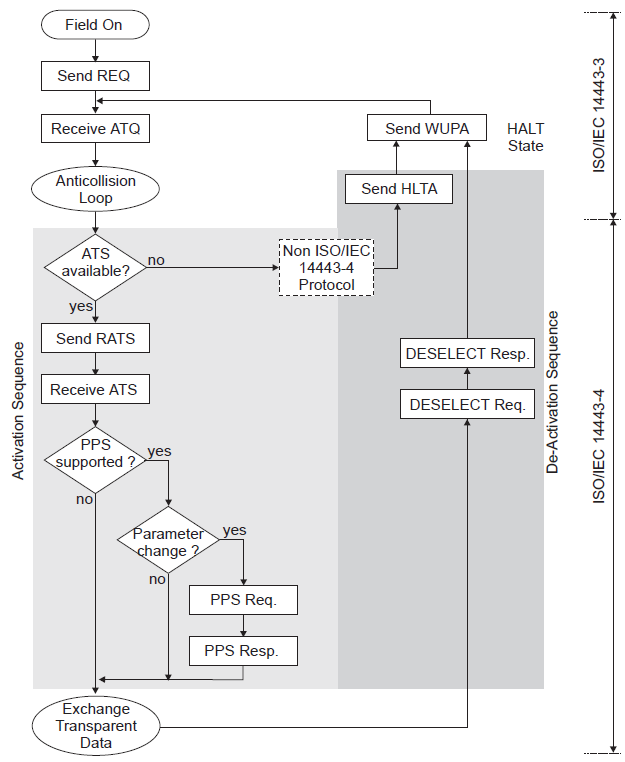
\includegraphics[width=6.27in,height=7.64in]{Norma_ISO/14443-4/media/image8.png}
    \end{center}
\end{figure}


%%%%%%%%%%%%%%%%%%%% Figure/Image No: 1 Ends here %%%%%%%%%%%%%%%%%%%%

\par
\begin{center}
\textbf{Figura 3.8.5.1 - Activación de un PICC Tipo A desde un PCD}
\end{center}
\par

\paragraph{Solicitud de respuesta para seleccionar}
Esta cláusula define las RATS con todos sus campos\par

El byte de parámetro consta de dos partes (figura 3.8.5.2):\par

El medio byte b8 a b5 más significativo se denomina FSDI y codifica FSD. El FSD define el tamaño máximo de una trama que el PCD puede recibir.\par

El medio byte menos significativo b4 a b1 se denomina CID y define el número lógico del PICC direccionado en el rango de 0 a 14. El valor 15 es RFU. El CID está especificado por el PCD y será único para todos PICCs, que están en el estado ACTIVO al mismo tiempo. El CID se fija por el tiempo que el PICC está activo y el PICC usará el CID como su identificador lógico, que está contenido en el primer RATS sin errores recibido.\par


\vspace{\baselineskip}


%%%%%%%%%%%%%%%%%%%% Figure/Image No: 2 starts here %%%%%%%%%%%%%%%%%%%%

\begin{figure}[H]
	\begin{center}
		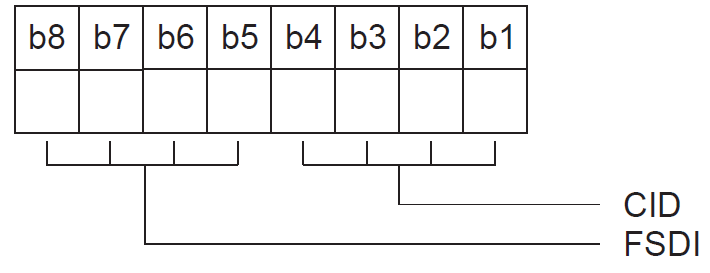
\includegraphics[width=3.84in,height=1.48in]{Norma_ISO/14443-4/media/image5.png}
    \end{center}
\end{figure}


%%%%%%%%%%%%%%%%%%%% Figure/Image No: 2 Ends here %%%%%%%%%%%%%%%%%%%%

\par
\begin{center}
\textbf{Figura 3.8.5.2 - Byte de parámetros del comando RATS.}
\end{center}
\par

\paragraph{Respuesta a SELECT}
Esta cláusula define el ATS con todos sus campos disponibles (Figura 3.8.5.3).\par

En el caso de que uno de los campos definidos no esté presente en un ATS enviado por un PICC, se aplicarán los valores predeterminados para ese campo.\par


\vspace{\baselineskip}


%%%%%%%%%%%%%%%%%%%% Figure/Image No: 3 starts here %%%%%%%%%%%%%%%%%%%%

\begin{figure}[H]
	\begin{center}
		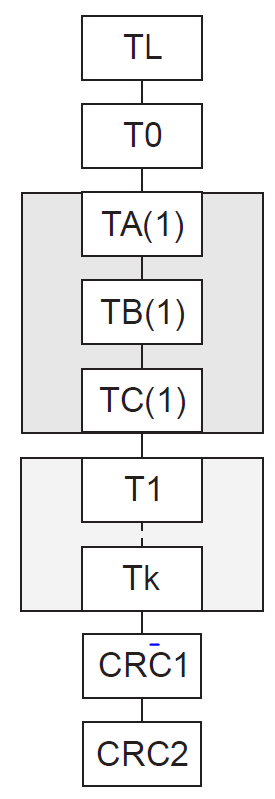
\includegraphics[width=0.88in,height=2.56in]{Norma_ISO/14443-4/media/image3.png}
    \end{center}
\end{figure}


%%%%%%%%%%%%%%%%%%%% Figure/Image No: 3 Ends here %%%%%%%%%%%%%%%%%%%%

\par

\begin{center}
\textbf{Figura 3.8.5.3 - Estructura del comando ATS.}
\end{center}
\par

\paragraph{Estructura de los bytes}
El byte de longitud TL viene seguido de un número variable de bytes posteriores opcionales en el siguiente orden:\par

\begin{itemize}
	\item formato de bytes T0,\par

	\item bytes de interfaz TA (1), TB (1), TC (1) y bytes históricos T1 a Tk.
\end{itemize}\par

\paragraph{Longitud de bytes}
El TL de longitud de bytes es obligatorio y especifica la longitud del ATS transmitido incluido él mismo. Los dos bytes CRC no están incluidos en TL. El tamaño máximo del ATS no debe exceder el FSD indicado. Por lo tanto, el valor máximo de TL no debe exceder el FSD-2.\par

\paragraph{Formato de byte}
El byte de formato T0 es opcional y está presente tan pronto como la longitud sea mayor que 1. El ATS solo puede contener los siguientes bytes opcionales, cuando este byte de formato está presente.\par

T0 consta de tres partes:\par

\begin{itemize}
	\item El bit más significativo b8 se establecerá en 0. El valor 1 es RFU.\par

	\item Los bits b7 a b5 indican la presencia de bytes de interfaz posteriores TA (1), TB (1) y TC (1).\par

	\item El medio byte menos significativo b4 a b1 se llama FSCI y codifica FSC. El FSC define el tamaño máximo de un marco aceptado por el PICC. El valor predeterminado de FSCI es 2 y conduce a un FSC de 32 bytes. La codificación de FSC es igual a la codificación de FSD.
\end{itemize}\par

\paragraph{Byte de interfaz TA (1)}
El byte de interfaz TA (1) consta de cuatro partes:\par

\begin{itemize}
	\item El bit más significativo b8 codifica la posibilidad de manejar diferentes divisores para cada dirección. Cuando este bit se establece en 1, el PICC no puede manejar diferentes divisores para cada dirección.\par

	\item Los bits b7 a b5 codifican la capacidad de tasa de bits del PICC para la dirección de PICC a PCD, llamada DS. El valor predeterminado será (000) b.\par

	\item El bit b4 se establece en (0) b y el otro valor es RFU.\par

	\item Los bits b3 a b1 codifican la capacidad de velocidad de bits del PICC para la dirección de PCD a PICC, llamada DR. El valor predeterminado será (000) b.
\end{itemize}\par

\paragraph{Byte de interfaz TB (1)}
El\ byte de interfaz TB (1) transmite información para definir el tiempo de espera de la trama y el tiempo de guarda  de la trama de inicio.\par

El byte de interfaz TB (1) consta de dos partes:\par

\begin{itemize}
	\item El medio byte b8 a b5 más significativo se denomina FWI y codifica FWT\par

	\item El medio byte menos significativo b4 a b1 se llama SFGI y codifica un valor multiplicador utilizado para definir el SFGT. El SFGT define un tiempo de protección específico que necesita el PICC antes de estar listo para recibir el siguiente cuadro después de haber enviado el ATS. SFG está codificado en el rango de 0 a 14. El valor de 15 es RFU. El valor de 0 indica que no se necesita SFGT y los valores en el rango de 1 a 14 se usan para calcular el SFGT con la fórmula que se indica a continuación. El valor predeterminado de SFG es 0.
\end{itemize}\par

\begin{center}
 \( SFGT= \left( 256\ast\frac{16}{fc} \right) \ast2^{SFG} \) 
\end{center}
\par

\paragraph{Bytes históricos}
Los bytes históricos T1 a Tk son opcionales y aportan información general. La longitud máxima de ATS da la cantidad máxima posible de bytes históricos. ISO / IEC 7816-4 especifica el contenido de los bytes históricos.\par

\paragraph{Petición de selección de protocolo y parámetro}
La solicitud de PPS contiene el byte de inicio seguido de un byte de formato y un byte de parámetro (figura 3.8.5.4).\par


\vspace{\baselineskip}


%%%%%%%%%%%%%%%%%%%% Figure/Image No: 4 starts here %%%%%%%%%%%%%%%%%%%%

\begin{figure}[H]
	\begin{center}
		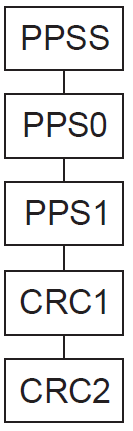
\includegraphics[width=0.53in,height=1.7in]{Norma_ISO/14443-4/media/image7.png}
    \end{center}
\end{figure}


%%%%%%%%%%%%%%%%%%%% Figure/Image No: 4 Ends here %%%%%%%%%%%%%%%%%%%%

\par
\begin{center}
\textbf{Figura 3.8.5.4 - Solicitud de selección de protocolo y parametros.}
\end{center}
\par

\paragraph{Inicio de selección de protocolo y parámetros}
El PPSS consta de dos partes:\par

\begin{itemize}
	\item El medio byte más significativo b8 a b5 es igual a 'D' e identifica el PPS.\par

	\item El medio byte menos significativo b4 a b1 se denomina CID y define el número lógico del PICC direccionado.
\end{itemize}\par

\paragraph{Selección 0 de protocolo y parámetros.}
El PPS0 consta de cuatro partes:\par

\begin{itemize}
	\item b8 a b6 deberá establecerse en (000)b, todos los demás valores son RFU\par

	\item b5 si el PPS1 es transmitido se establece en (1)b.\par

	\item b4 a b2 deberá establecerse en (000)b, todos los demás valores son RFU\par

	\item b1deberá establecerse en (1)b, (0)b es RFU
\end{itemize}\par

\paragraph{Selección 1 de protocolo y parámetros.}
El PPS1 consta de tres partes:\par

\begin{itemize}
	\item El medio byte más significativo b8 a b5 es (0000) b y todos los demás valores son RFU.\par

	\item Los bits b4, b3 se llaman DSI y codifican el divisor entero seleccionado de PICC a PCD.\par

	\item Los bits b2, b1 se llaman DRI y codifican el divisor entero seleccionado de PCD a PICC.
\end{itemize}\par

\paragraph{Respuesta de selección de protocolo y parámetros}
La respuesta de PPS confirma la solicitud de PPS recibida.\par

\paragraph{Tiempo de espera de la trama de activación}
El tiempo de espera de la trama de activación define el tiempo máximo para que un PICC comience a enviar su trama de respuesta después del final de una trama recibida del PCD y tiene un valor de 65536 / fc ($ \sim $  4833 $ \mu $ s).\par

\paragraph{Detección y recuperación de errores}
\paragraph{Manejo de RATS y ATS}
\paragraph{Reglas de PCD}
Cuando el PCD ha enviado el RATS y recibe un ATS válido, el PCD continuará funcionando.\par

En cualquier otro caso, el PCD puede retransmitir la RATS antes de que utilice la secuencia de desactivación tal como se define en la cláusula 8.\par

\paragraph{Reglas del PICC}
Cuando el PICC ha sido seleccionado con el último comando y\par

\begin{enumerate}
	\item Recibe un RATS válido, el PICC deberá\par

\begin{itemize}
	\item enviar de vuelta su ATS y\par

	\item deshabilitar las RATAS (no responda más a las RATS recibidas).
\end{itemize}\par

	\item Recibe cualquier otro bloque válido o inválido, excepto un comando HLTA, el PICC deberá
\end{enumerate}\par

\begin{itemize}
	\item ignorar el bloque y permanezca en modo de recepción.
\end{itemize}\par

\paragraph{Tratamiento de solicitud PPS y respuesta PPS}
\paragraph{Reglas del PCD}
Cuando el PCD ha enviado una solicitud de PPS y recibió una respuesta de PPS válida, el PCD activará los parámetros seleccionados y continuará la operación.\par

En cualquier otro caso, el PCD puede retransmitir una solicitud de PPS y continuar la operación.\par

\paragraph{Reglas de PICC }
Cuando el PICC ha recibido un RATS, envía su ATS y\par

\begin{enumerate}
	\item 1. recibió una solicitud de PPS válida, el PICC deberá\par

\begin{itemize}
	\item envía la respuesta de PPS,\par

	\item deshabilitar la solicitud de PPS (ya no responde a las solicitudes de PPS recibidas) y\par

	\item activar el parámetro recibido.
\end{itemize}\par

	\item Recibió un bloque inválido, el PICC deberá\par

\begin{itemize}
	\item deshabilitar la solicitud de PPS (ya no responde a las solicitudes de PPS recibidas) y\par

	\item permanecer en modo de recepción.
\end{itemize}\par

	\item Recibió un bloque válido, excepto una solicitud de PPS, el PICC deberá
\end{enumerate}\par

\begin{itemize}
	\item deshabilitar la solicitud de PPS (ya no responde a las solicitudes de PPS recibidas) ycontinuar operando
\end{itemize}\par

\paragraph{Manejo del CID durante la activación}
Cuando el PCD ha enviado un RATS que contiene un CID = n distinto a 0 y\par

\begin{enumerate}
	\item Recibió un ATS que indica que el CID es compatible, el PCD deberá\par

\begin{itemize}
	\item enviar bloques que contengan CID = n a este PICC\par

	\item no usar el CID = n para RATS adicionales mientras este PICC esté en estado ACTIVE.
\end{itemize}\par

	\item Recibió un ATS que indica que el CID no es compatible, el PCD deberá enviar bloques que no contengan CID a este PICC y no activar ningún otro PICC mientras este PICC esté en estado ACTIVE.
\end{enumerate}\par

Cuando el PCD ha enviado un RATS que contiene un CID igual a 0 y\par

\begin{enumerate}
	\item Recibió un ATS que indica que CID es compatible, el PCD puede\par

\begin{itemize}
	\item enviar bloques que contengan CID igual a 0 a este PICC\par

	\item no activar ningún otro PICC mientras este PICC esté en estado ACTIVE.
\end{itemize}\par

	\item Recibió un ATS que indica que el CID no es compatible, el PCD deberá
\end{enumerate}\par

\begin{itemize}
	\item enviar bloques que no contengan CID a este PICC y no activar ningún otro PICC mientras este PICC esté en estado ACTIVE.
\end{itemize}\par




\clearpage
\section{Antecedentes del proyecto}
\label{sec:antecedentes}
En esta sección se describe el diseño y desarrollo de cada etapa del proyecto desde 2015 hasta la actualidad. Dichos avances pueden encontrarse en \cite{Proyecciones_0417} y \cite{Proyecciones_1017}, publicaciones realizadas durante el trabajo en los Proyectos de Investigación y Desarrollo dirigidos por el Ing. Sebastián Verrastro:
\begin{itemize}
\item Diseño y testing de circuitos integrados de bajo consumo para aplicaciones médicas implantables.
\item Investigación y desarrollo de un circuito 
integrado transceptor por radio frecuencia, 
pasivo y de bajo consumo.
\end{itemize}

\subsection{Modulador} \label{subsec:modulador}
\subsubsection{Diseño del modulador de carga}
La comunicación desde la PICC hacia el PCD se lleva a cabo mediante variaciones en la carga del primer dispositivo, lo que genera, a su vez, variaciones de tensión en el segundo. Esta forma de comunicación es conocida como modulación de carga. Las variaciones de tensión dependen, principalmente, del nivel de acoplamiento existente entre ambos dispositivos, de la topología del modulador escogida y de los valores de componentes usados en la topología elegida.
A través de la modulación de carga, se generan bandas laterales de modulación en el espectro (Figura \ref{fig:Mod_carg}). Si se generan variaciones con una frecuencia alta $f_s$, se crean dos líneas espectrales a una distancia $\pm f_s$ alrededor de la frecuencia de transmisión del PCD.
Las variaciones de tensión que se observan en el PCD son características propias de la modulación por desplazamiento de amplitud que se genera a través de las variaciones de la carga en el PICC. La ASK se caracteriza por desarrollarse a través de la variación de la señal portadora entre dos valores de amplitud, es decir, entre dos estados, a una frecuencia $f_s$. La modulación ASK tiene características similares a la muy conocida modulación AM (modulación de amplitud). Como esta última, la ASK es lineal, sencilla de implementar y la reconstrucción de los datos enviados es relativamente simple.

\begin{figure}[H]
\centering
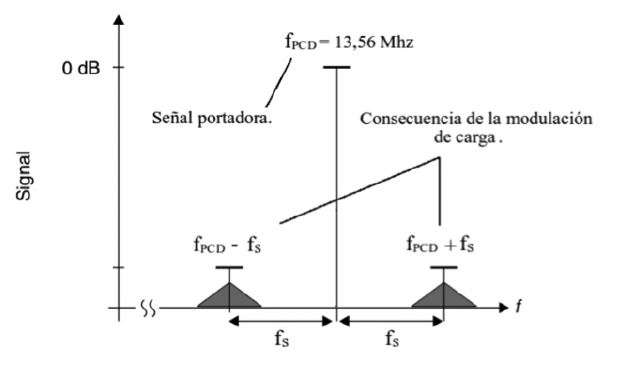
\includegraphics[scale=0.5]{Antecedentes/Modulacion_Carga.JPG}
\caption{Modulación de carga.}
\label{fig:Mod_carg}
\end{figure}


Los moduladores constan de dos transistores
NMOS que se abren y se cierran dependiendo
del valor de tensión que se aplica en la compuerta
de estos. Como se mencionó anteriormente,
la modulación en amplitud maneja dos
estados de tensión, entonces, los transistores
estarán al corte o conduciendo, provocando
una conmutación de carga en paralelo al circuito
resonante.

\begin{figure}[H]
\centering
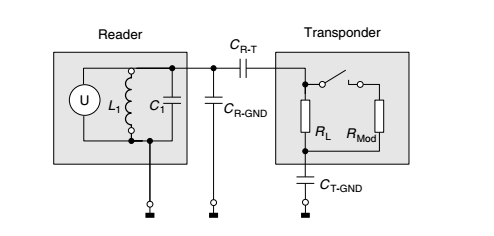
\includegraphics[scale=0.5]{Antecedentes/Modulador_Equiv.png}
\caption{Equivalente del modulador de carga.}
\label{fig:Mod_equ}
\end{figure}

\subsubsection{Modulador Capacitivo}
Analizando las distintas formas de realizar la
modulación de carga, se tomó como primer
circuito a analizar una topología de modulación
capacitiva presentada en la Figura \ref{fig:Mod_carg_cap}. El
funcionamiento de este módulo consta del
agregado (en uno de los estados de $V_Data$) de
capacitores en paralelo al circuito resonante
del PICC, mientras que, en el otro nivel lógico,
el circuito resonante no se ve afectado. Esta
variabilidad de capacidad provoca una mínima
desintonía entre los dispositivos, lo cual influye
en la transferencia de energía entre estos y se
observa como una variación en la tensión observada
en la antena del PCD.
Se realizó, inicialmente, el análisis del comportamiento
del modulador con el equivalente
en pequeña señal de los transistores debido a
que se manejó la posibilidad de que las capacidades
parásitas de estos afecten al circuito
modulador. Finalmente, se corroboró que estas
capacidades no afectan el funcionamiento
del módulo y se realizaron simulaciones para
obtener los valores correctos de $C_1$ y $C_2$ para
realizar una modulación con el mayor índice
de modulación posible. En las simulaciones se
tuvieron en cuenta los valores posibles de integración
para la tecnología. Vale aclarar que, 
a la hora de la integración, los capacitores
ocupan mucha área de silicio por lo que esto
acota los valores de capacidad con los cuales
disponemos para realizar el módulo a valores
menores o alrededor a la decena de pico faradios.
Con los valores de capacidad posibles ya
detectados, se hicieron análisis en frecuencia
para poder observar la “desintonía” que genera
esta topología para lograr la modulación.

\begin{figure}[H]
\centering
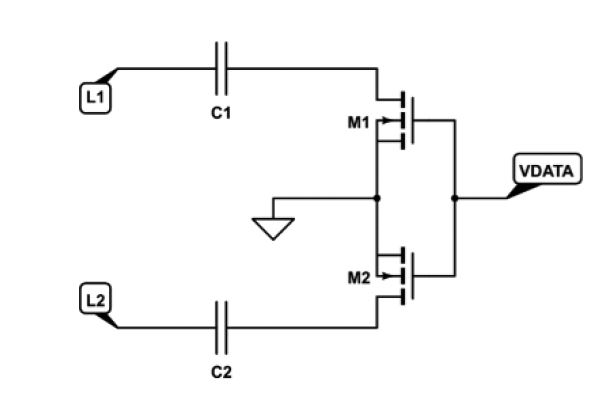
\includegraphics[scale=0.5]{Antecedentes/Modulacion_Carga_Cap.JPG}
\caption{Modulador de carga capacitivo.}
\label{fig:Mod_carg_cap}
\end{figure}

\subsubsection{Modulador óhmico con sólo transistores}
Buscando un mayor índice de modulación (en
este aspecto el modulador capacitivo es débil)
se analizó una topología de modulación óhmica,
en la cual se utiliza la resistencia de salida
propia de los NMOS (Figura \ref{fig:Mod_carg_trans}). 
Al ser
una impedancia baja, cuando se encuentra en
paralelo al circuito resonante y a la carga que
conforman los demás módulos que se encuentran
conectados a este circuito, la impedancia
del conjunto baja considerablemente. Si se varía 
la puesta en paralelo de la impedancia de
salida de los NMOS a la frecuencia $f_s$, se obtiene
una modulación de carga.
A través de la simulación de la topología de
la Figura \ref{fig:Mod_carg_trans}, se observó lo buscado: un índice
de modulación considerablemente mayor al
obtenido anteriormente. En el análisis enfocado
hacia los transistores y su comportamiento
durante la modulación, se detectaron picos
de corriente (Figura \ref{fig:Picos_Cor}), en el drain
de cada uno de los transistores, que podrían
afectar a estos dispositivos luego de un uso
considerable de estos. Estos picos se generan
debido a que, en las simulaciones, los tiempos
de rise (subida) y fall (bajada) de la señal
$V_Data$ son de valores muy pequeños. Si bien
en el uso empírico de los dispositivos estos
valores suelen ser mayores, lo que provocaría
disminución en los picos nombrados, se procedió
a buscar un margen de seguridad en el circuito.
\begin{figure}[H]
\centering
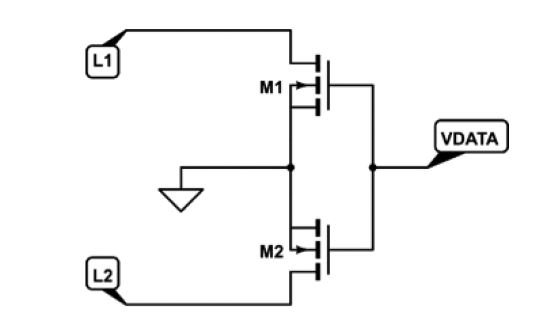
\includegraphics[scale=0.5]{Antecedentes/Modulacion_Carga_Trans.JPG}
\caption{Modulador de carga óhmico.}
\label{fig:Mod_carg_trans}
\end{figure}

\begin{figure}[H]
\centering
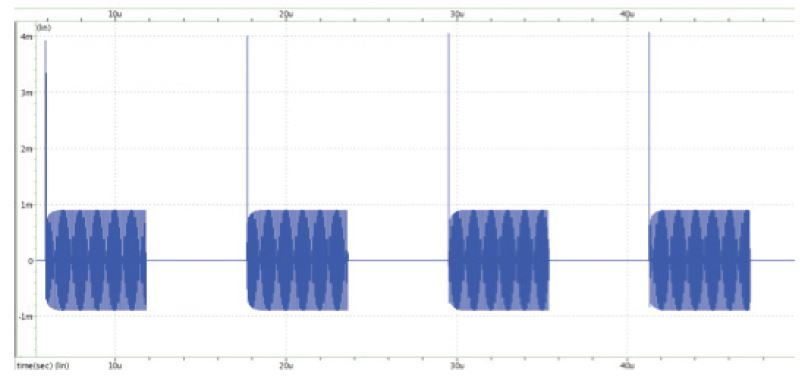
\includegraphics[scale=0.5]{Antecedentes/Picos_Corriente.JPG}
\caption{Corriente en el drain del NMOS M2 en la topología sin capacitores ni resistores.}
\label{fig:Picos_Cor}
\end{figure}


\subsubsection{Modulador óhmico con resistores}
Buscando la protección de los transistores
ante picos de corrientes inesperados se
modificó la topología de la Figura 8 mediante
el uso de dos resistores que protejan los
drenajes de los NMOS pero que, a su vez, no
disminuyan considerablemente la modulación
obtenida con la topología anterior. El nuevo
circuito quedó conformado como se muestra
en la Figura \ref{fig:Mod_carg_res}.
Para encontrar el valor de capacidades en la
topología de la Figura \ref{fig:Mod_carg_cap} se habían tenido en
cuenta ciertos parámetros deseados. Con los
resistores se trabajó de forma similar, pero
enfocando el diseño en otros parámetros. Se
buscaron valores de resistencias que realicen
una protección correcta de los transistores y
que, a su vez, no afecten de forma considerable
al índice de modulación logrado con la
topología de la Figura \ref{fig:Mod_carg_trans}.
Luego de verificar que los picos de corrientes
en los drenajes de los NMOS eran considerablemente
menores a los vistos en la topología
anterior y que la modulación generada en el
circuito resonante del PCD mantenía un buen
índice de modulación, se continuó con los análisis
a esta topología.
Uno de los problemas que pueden surgir en los
circuitos electrónicos son los comportamientos
indeseados debido a variaciones e incertidumbres
en los componentes que componen los
circuitos. Para asegurarse que, ante estas variaciones,
el circuito seguirá funcionando como
se desea, es que se realizan las simulaciones
con el método de Montecarlo. Este método
consiste en realizar un análisis estadístico numérico
analizando el comportamiento del circuito
ante variaciones probabilísticas en sus
componentes. Realizando estas simulaciones
para variaciones de los valores nominales de
los resistores $R_1$ y $R_2$ nos aseguramos que el
circuito mantenga su correcto funcionamiento
en el caso de alteraciones en estos.
Para aumentar nuestro margen de funcionabilidad,
el circuito se sometió a simulaciones
mediante corners (extremos del proceso) que
contienen las posibles variaciones en las características
de los transistores provocadas por el
proceso de fabricación del CI.

\begin{figure}[H]
\centering
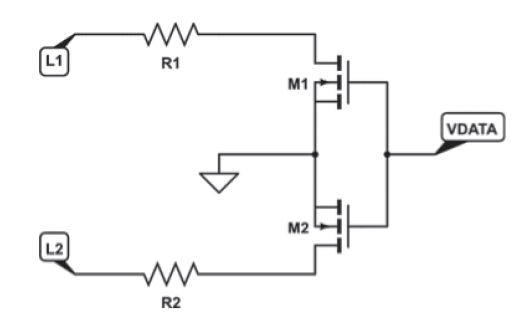
\includegraphics[scale=0.5]{Antecedentes/Modulacion_Carga_Res.JPG}
\caption{Modulador de carga óhmico con resistores.}
\label{fig:Mod_carg_res}
\end{figure}

A continuación, en la fig. \ref{fig:prof_moduladores}, se muestra uno de los factores usados para comparar las distintas topologías.

\begin{figure}[H]
 \centering
  \subfloat[Modulador capacitivo.]{
   \label{f:prof_cap}
    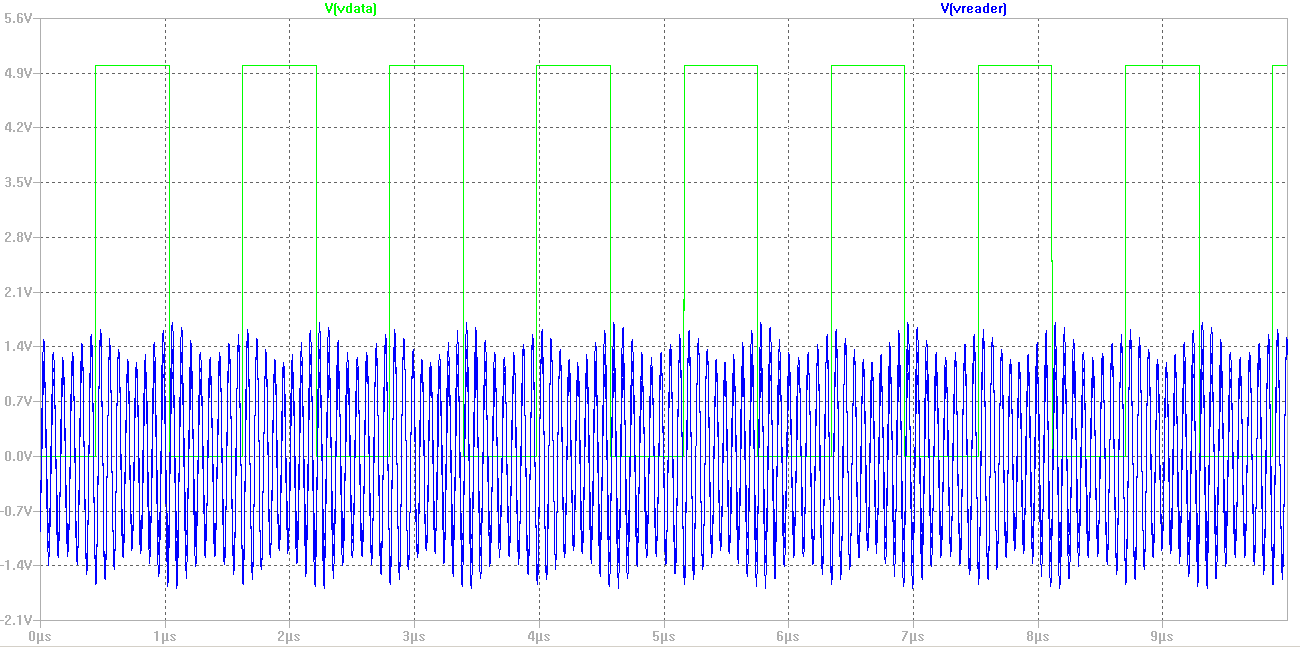
\includegraphics[width=0.5\textwidth]{Antecedentes/Load_Modulation_Cap_Vreader.png}}
  \subfloat[Modulador óhmico sin resistores.]{
   \label{f:prof_trans}
    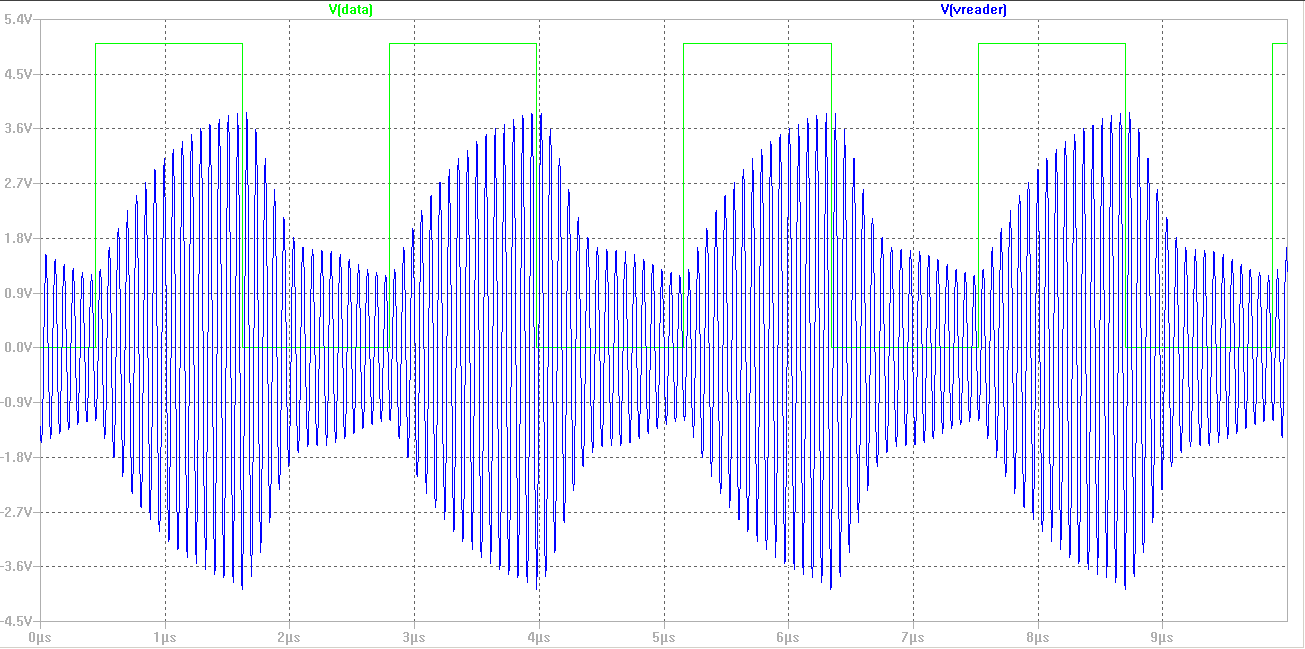
\includegraphics[width=0.5\textwidth]{Antecedentes/Load_Modulation_2_VReader.png}}
    \newline
  \subfloat[Modulador óhmico con resistores.]{
   \label{f:prof_res}
    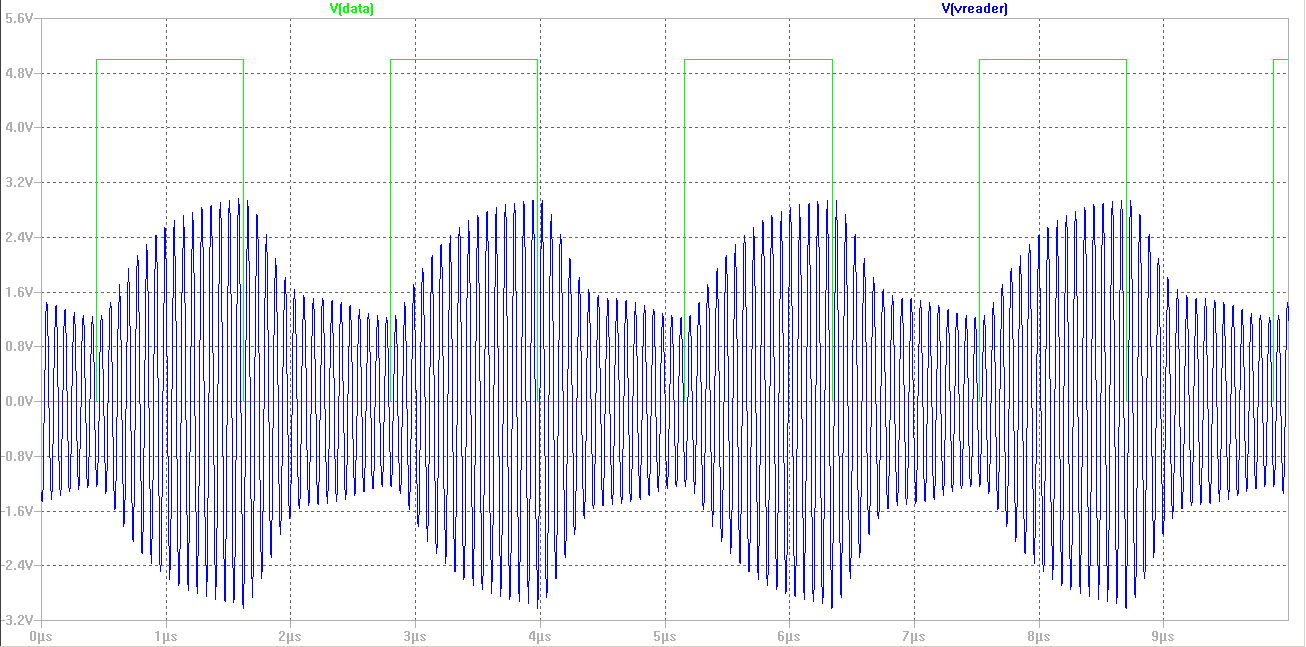
\includegraphics[width=0.5\textwidth]{Antecedentes/LoadModulation1_Reader.png}}
 \caption{Profundidad de modulación de las diferentes topologías de modulador.}
 \label{fig:prof_moduladores}
\end{figure}


\subsection{Demodulador} \label{subsec:demodulador}
La comunicación desde el PCD al PICC se lleva a cabo mediante una
modulación ASK al 100\% con una codificación Miller Modificado
(Norma ISO14443 Tipo A). La modulación ASK
tiene como característica la variación de la señal
portadoras entre dos valores definidos. En
una modulación ASK al 100\%, la señal variará
entre un nivel de tensión mayor a cero y 0V
(cero Volt).
Se utilizaron varias topologías de demoduladores.
En la primer topología, la demodulación de la señal recibida en el
PICC, se llevó a cabo a través de varias etapas \ref{fig:Demo}. En primer lugar, se realizó la rectificación
de la señal y la detección de envolvente.
En una segunda etapa, se filtró la señal obtenida
en la etapa anterior para evitar errores en
la próxima fase de tratamiento de señal debido
a variaciones de alta frecuencia sobre la señal
envolvente. En la última parte, se ingresó la
señal ya filtrada a un Schmitt trigger \cite{schmitt} para obtener, a la salida, la señal
que representa los datos enviados por el PCD.
\begin{figure}[H]
\centering
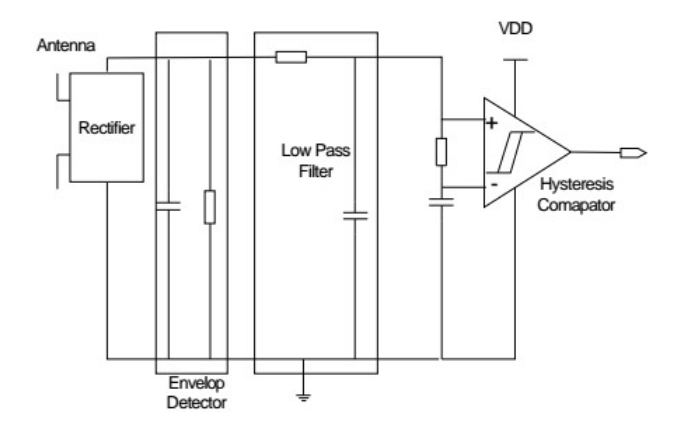
\includegraphics[scale=0.5]{Antecedentes/Demodulador.png}
\caption{Estructura básica de un demodulador \cite{RFID_Tuto}.}
\label{fig:Demo}
\end{figure}
La segunda topología utilizada (fig \ref{fig:Demod2}), además de estar conformada
por el Schmitt trigger y un filtro pasabajos,
posee en el diseño, un comparador y una entrada
de habilitación. Ésta tiene la ventaja de
poder ajustar el nivel del comparador externamente.
La desventaja es que el amplificador
operacional diseñado tiene un tiempo de
respuesta (Slew Rate) mucho mayor que el
Schmitt trigger.

\begin{figure}[H]
\centering
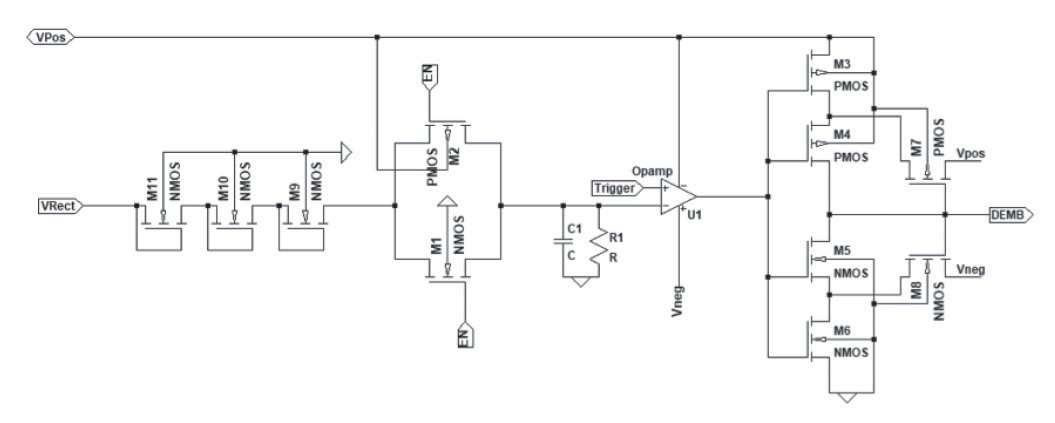
\includegraphics[scale=0.5]{Antecedentes/Demod2.PNG}
\caption{Esquemático de la segunda topología de demodulador utilizada.}
\label{fig:Demod2}
\end{figure}

\subsubsection{Rectificador y detector de envolvente}
En esta etapa se usó una topología típica de
un demodulador de AM (amplitud modulada),
la cual se ve en la Fig.\ref{fig:Detect} y se caracteriza
por ser un circuito simple, compuesto por un
rectificador y un detector (Resistor y Capacitor
en paralelo).
\begin{figure}[H]
\centering
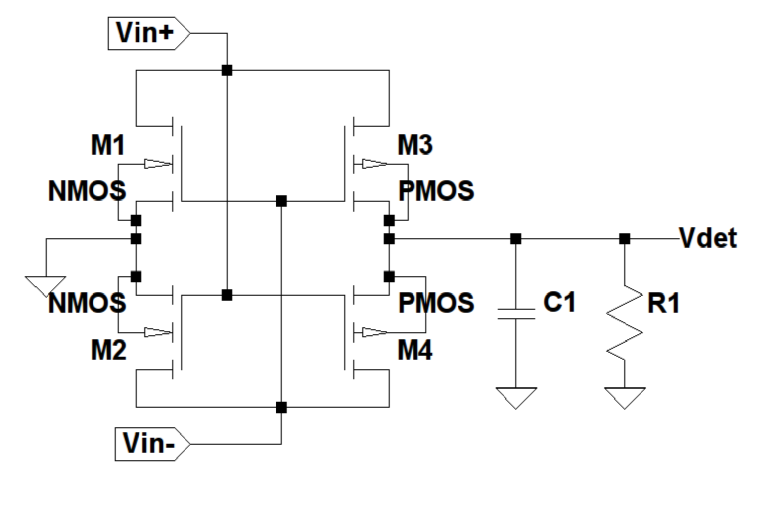
\includegraphics[scale=0.3]{Antecedentes/Detect_RC.png}
\caption{Rectificador y detector de envolvente.}
\label{fig:Detect}
\end{figure}
A continuación, se realizó el análisis matemático
de la topología para obtener los valores de
componentes que optimizan el funcionamiento
del circuito. Para un análisis más sencillo, se
optó por tomar como rectificador a un diodo.
Teniendo en cuenta que el detector de envolvente
se compone de un resistor y un capacitor, éste presenta una constante de tiempo $\tau = RC$.
Considerando también que se tiene una señal
portadora con una frecuencia igual a $f_c =
13,56 MHz$, el capacitor se descarga, entre
cada pico de portadora, siguiendo la siguiente
ecuación:
$$V'_{pico} = V_{pico}e^{-\frac{t}{\tau}}$$
Donde $T = \frac{1}{fc}$. Si tomamos $T << \tau$, entonces:
$$\bigtriangledown V \simeq V{pico}\frac{T}{\tau} = \frac{V_{pico}}{f_c \tau}$$

Cuando la señal está modulada en ASK, su
tensión pasa, de un valor de tensión definido
a un valor mucho menor (cero Volts en nuestro
caso). La caída de tensión en el detector
de envolvente, desde un valor a otro, se ve en la siguiente ecuación:
$$V_{caida} = V_{pico}e^{-\frac{t}{\tau}}$$

Desde la ecuación anterior, puede analizarse
el comportamiento del circuito detector ante el
cambio de tensión mencionado. Dependiendo
del \tau del RC, éste será más o menos sensible al
cambio de tensión.
Buscando, en la práctica, una buena relación
en la respuesta del circuito detector ante el
cambio de tensión a la frecuencia modulante
y ante el ripple a la frecuencia portadora, se
toma un \tau dentro del intervalo de la ecuación
siguiente:
$$\frac{1}{f_c} << \tau << \frac{1}{f_m}$$
Entonces, teniendo 13,56 MHz como $f_c$ (frecuencia
de portadora) y 106 kHz como $f_m$ (frecuencia
modulante) se escogieron los siguientes
valores de componente:
$$R = 5 k\Omega ; C = 30 pF$$
Quedándonos la siguiente relación entre frecuencias
y \tau:
$$\frac{1}{13.56MHz}<<1.5.10^{-7}s<<\frac{1}{106kHz}$$

\begin{figure}[H]
\centering
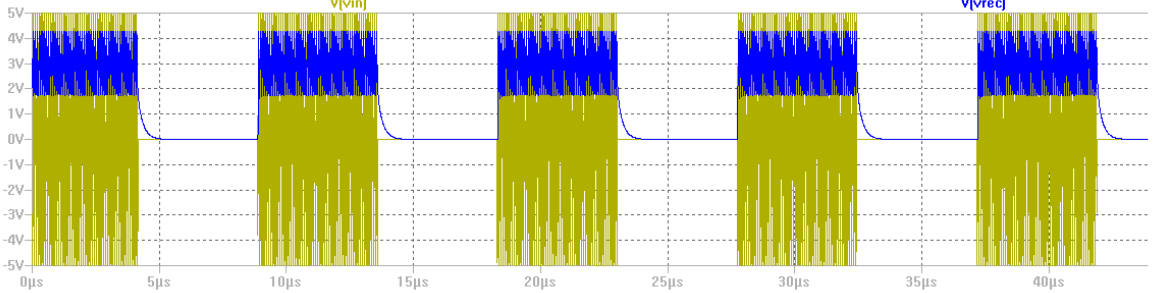
\includegraphics[scale=0.3]{Antecedentes/Sim_Detect.png}
\caption{Señal de entrada y señal de salida del detector de envolvente \tau = 0,15\mu S.}
\label{fig:Sim_detect}
\end{figure}

\subsubsection{Filtro pasa bajos}
Una vez que, la señal modulada que llega al
PICC, pasa por el detector de envolvente, ésta,
queda con un ripple a la frecuencia de la portadora.
Para evitar que en la siguiente etapa se
produzcan fallas debido a variaciones de tensión
no deseadas, la señal de salida del detector,
pasa por un filtro RC (pasa bajos simple) cuyo
fin es mitigar las ondulaciones a 13,56 MHz.
La frecuencia de corte del filtro deberá estar por
debajo de la frecuencia de portadora, para así
filtrarla y por encima de la frecuencia modulante,
para no afectar la envolvente. Entonces:
$$\frac{1}{106kHz}<<f_c<<\frac{1}{13.56MHz}$$
$$f_c = \frac{1}{2\pi RC} \approx 3.2MHz$$
$$R = 10 k\Omega ; C = 6 pF$$

\begin{figure}[H]
\centering
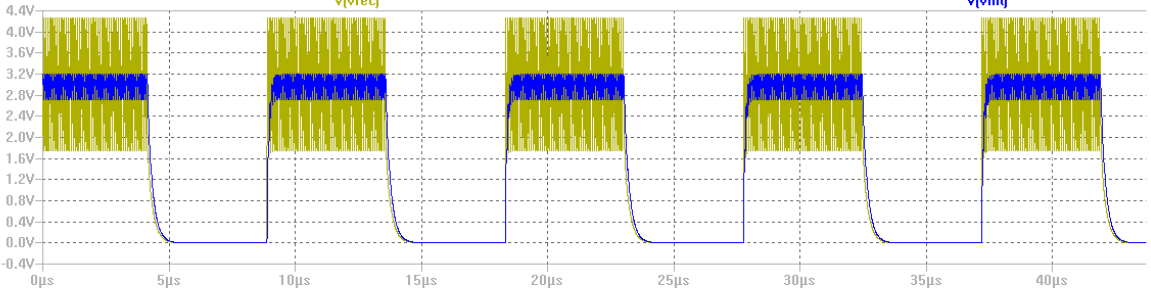
\includegraphics[scale=0.3]{Antecedentes/Sim_RC.png}
\caption{Filtrado del riple de 13.56MHz con filtro RC.}
\label{fig:Sim_RC}
\end{figure}

\subsubsection{Schmitt trigger}
Dado que la señal de salida del demodulador
ingresará luego a un sistema digital, ésta debe
estar libre de ruido y distorsiones para evitar
errores en la información y, por lo tanto, en el
sistema encargado del manejo de la información.
Una forma de digitalizar una señal, eliminando
las perturbaciones que trae, es a través
de un Schmitt trigger.
Este tipo de disparador se caracteriza por su
naturaleza biestable y por el uso de una histéresis
que gobierna los cambios de estados. La
topología escogida es la de un inversor CMOS
de doble transistor con la adición de un par de
transistores que son los que definen los puntos
de cambio de estado en la histéresis.
Esta topología, cuenta con la ventaja de poder
escoger los puntos de disparo del sistema eligiendo
la relación de aspecto de los transistores que la conforman. 
Las relaciones entre el ancho
y el largo del canal de los transistores, tienen
efecto en la histéresis del disparador.

\begin{figure}[H]
\centering
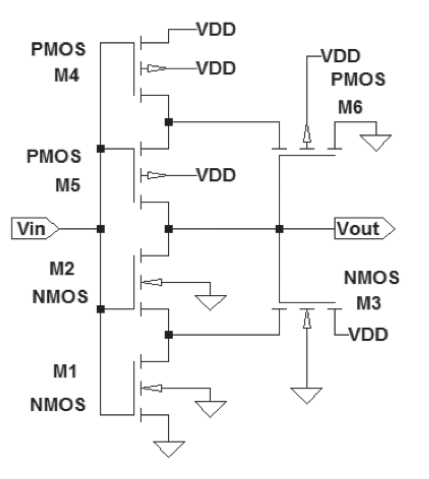
\includegraphics[scale=0.5]{Antecedentes/Schmitt_Trigger.PNG}
\caption{Schmitt Trigger CMOS.}
\label{fig:Schmit}
\end{figure}

Cuando en la entrada del circuito (Fig. \ref{fig:Schmit}) hay
0 V, los transistores $M_4$ y $M_5$, estarán conduciendo,
mientras que el $M_1$ y el $M_2$, estarán en
corte. Con esa condición, la salida estará en alto
($V_{out} = V_{DD}$). Cuando la tensión de entrada comience
a subir y alcance la tensión de umbral
del transistor $M_1$, éste comenzará a conducir,
pero el $M_2$ se mantendrá apagado. El $M_1$ tenderá
a hacer bajar el nodo entre éste y el $M_2$ a
GND, mientras que, el $M_3$, que tiene $V_{DD}$ en su
gate, hará tender el nodo hacia $V_{DD}$. Cuando la
señal de entrada supere la tensión umbral del
$M_2$, entonces, éste comenzará a conducir y la
salida tendrá 0V de tensión, denominando la
tensión de entrada que dispara la salida al nivel
bajo como $V_{IH}$ (tensión límite que se admite
como uno lógico).
Algo similar ocurre con la rama superior del inversor
cuando la tensión de entrada comienza a
disminuir. Los transistores $M_4$ y $M_6$ harán tender
el nodo hacía VDD y GND respectivamente,
hasta que el $M_5$ comience a conducir y la salida
pase al estado alto, denominando, entonces, la
tensión de entrada que dispara la salida al nivel
alto como $V_{IL}$ (tensión límite que se admite
como cero lógico).
Partiendo del análisis en condiciones de saturación
de los transistores $M_1$ y $M_3$ se llegó a la
expresión de la $V_{IH}$ en función de las relaciones
de aspecto de dichos transistores:
$$I_{DM3} = \frac{\beta _3}{2(V_{GS}-V_{TH3})^2}$$
Siendo:
$$\beta = \mu _n C_{ox} (\frac{W}{L})^2 $$
Donde $\mu _n$ e la movilidad de los electrones en el silicio, $C_ox$ es la capacidad del Óxido, W el ancho de la compuerta
del transistor y L el largo de la compuerta del transistor.

Desarrollando y teniendo en cuenta que:
$$V_{TH2} = V_{TH2};  I_{DM3} = I_{DM1}$$
Puede llegarse a la siguiente expresión:
$$V_{IH}= \frac{V_{DD}+V_{VTH1}\sqrt[]{\frac{\beta _1}{\beta _3}}}{1+\sqrt[]{\frac{\beta _1}{\beta _3}}}$$

Haciéndose un análisis similar, pero en condiciones
de saturación para los transistores $M_6$ y $M_4$, se
llega a la expresión de VIL:
$$I_{DM6} = \frac{\beta _6}{2(V_{SG}-|V_{TH6}|)^2}$$

Desarrollando y teniendo en cuenta que:
$$V_{TH5} = V_{TH6};  I_{DM4} = I_{DM6}$$
Puede llegarse a la siguiente ecuación:
$$V_{IL}= \frac{\sqrt[]{(\frac{\beta _4}{\beta _6})(V_{DD}-|V_{TH4}|)}}{1+\sqrt[]{\frac{\beta _4}{\beta _6}}}$$
Una vez encontradas las expresiones de $V_{IL}$ y
$V_{IH}$, se buscó una relación entre los tamaños de
los transistores, para lograr un óptimo funcionamiento
del circuito, evitando errores por ruido
de alta frecuencia y distorsiones en la señal de
entrada.

\begin{figure}[H]
\centering
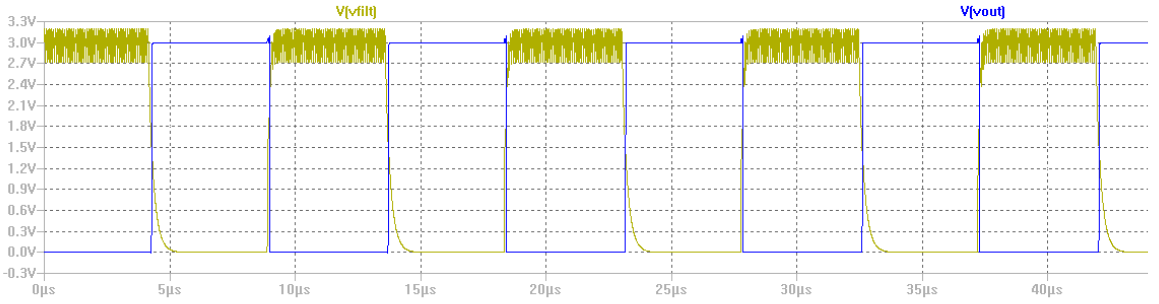
\includegraphics[scale=0.3]{Antecedentes/Sim_Schmit.png}
\caption{Tensión de entrada y de la salida del Schmitt Trigger.}
\label{fig:Sim_Schmit}
\end{figure}

Como resultado de todas las etapas mencionadas anteriormente, se obtuvo un demodulador que opera según la fig. \ref{fig:Sim_demo}.

\begin{figure}[H]
\centering
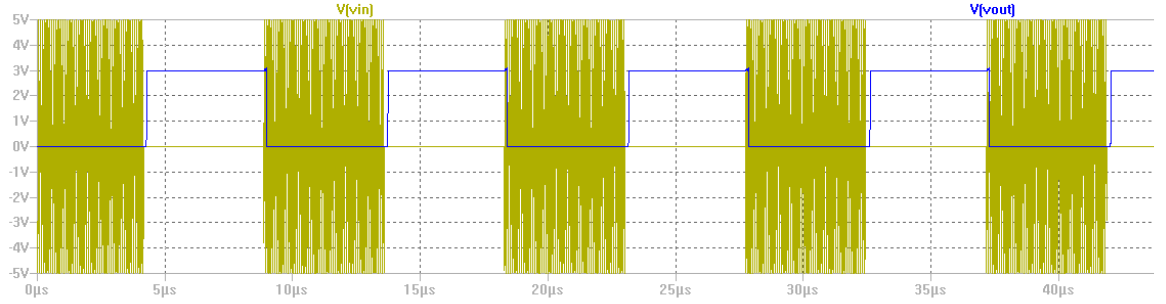
\includegraphics[scale=0.3]{Antecedentes/Sim_Demo.png}
\caption{Tensión de entrada y de la salida del demodulador.}
\label{fig:Sim_demo}
\end{figure}



\subsection{Limitador (Shunt)} \label{subsec:limit}

Se eligieron dos topologías de limitador Shunt, la primera topología se basó en el de Zheng Zhu \cite{shunt1}, y la segunda topología en Napong Panitantu \cite{shunt2}.

Al final se implementó en el desarrollo final la topología de Napong, ya que los resultados fueron más óptimos \cite{Proyecciones_1017}. En la figura \ref{fig:shunt2} se muestra la topología.

\begin{figure}[H]
\centering
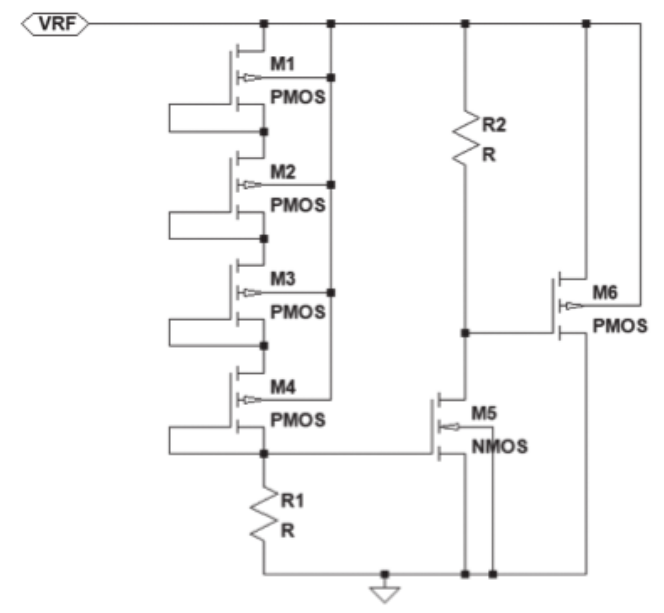
\includegraphics[width=0.4\linewidth]{circuitos/Shunt_2.png}
\caption{Limitador de potencia - Shunt}
\label{fig:shunt2}
\end{figure}

Siendo:

$$Vgs_{6} > Vth_{p}$$

lo que ocurre cuando el transistor M5 se encuentra en saturación. Dicha situación se logra cuando la tensión sobre el gate del transistor M5 es:

$$Vgs_{6} = Vrf - Vds_{5}$$
$$Vgs_{5} > (Vrf - Vgs_{1} + Vgs_{2} + Vgs_{3} + Vgs_{4}) $$

En función de esto se diseñó la topología para que a partir de los 6 V (para el caso de ONC5) comience a operar el transistor M6. En las figuras \ref{fig:shunt_500} y \ref{fig:shunt_500} se observan resultados obtenidos en la simulación de este módulo.

\clearpage
\section{Marco Teórico - Antena}
\label{sec:antena}
\subsection{Base y principio de diseño}
La aplicación fundamental de las antenas es la transmisión y recepción de información empleando, para ello, radiación electromagnética. También, como es el caso de la tecnología RFID utilizada en el proyecto, una de las antenas (PICC) toma energía del flujo magnético generado por la otra (PCD), energizandose.

Para lograr el cumplimiento de la norma sobre RFID ISO 14443 Tipo A logrando, así, la comunicación entre el PCD y el PICC se deben tener en cuenta las características de la comunicación:

\begin{itemize}
\item Frecuencia de portadora.
\item Frecuencia de subportadoras.
\item Modulación ASK 100\% desde el PCD al PICC.
\item Modulación de carga desde el PICC al PCD.
\end{itemize}

Además de las características que debe tener una antena ante la transmisión de información, se debe tener en cuenta la distancia entre antenas entre las cuales es alcanzable el funcionamiento de la comunicación, para este factor de los sistemas RFID, se debe tener en cuenta:

\begin{itemize}
\item Tamaño de antena PCD (y PICC)
\item Emparejamiento de la antena
\item Factor de calidad de la antena y circuito de adaptación
\item Potencia de la PCD
\item Influencias medioambientales
\end{itemize}

\subsection{Funcionamiento del sistema}

La corriente en la antena del PCD genera un flujo magnético Φ. Partes de este flujo Φ fluye a través de la bobina de la tarjeta e induce un voltaje. Esta tensión se rectifica y el IC de la tarjeta se activa cuando se alcanza la tensión de funcionamiento.
El voltaje inducido variará dentro de la distancia entre la antena PCD y el PICC. Debido a esa variación, la distancia de operación alcanzable está limitada por la potencia transferida.

Basado en el principio del transformador (Figura \ref{fig:trafo}) y en la leyes de Faraday para electromagnetismo, puede calcularse la densidad media del flujo y así la tensión inducida en dependencia del ángulo de operación, el radio y espiras de la antena del PICC. Basándose, además, en el límite de la intensidad de campo mínima requerida como se especifica en ISO14443-2 (Sección \ref{sec:iso}).

\begin{figure}[H]
\centering
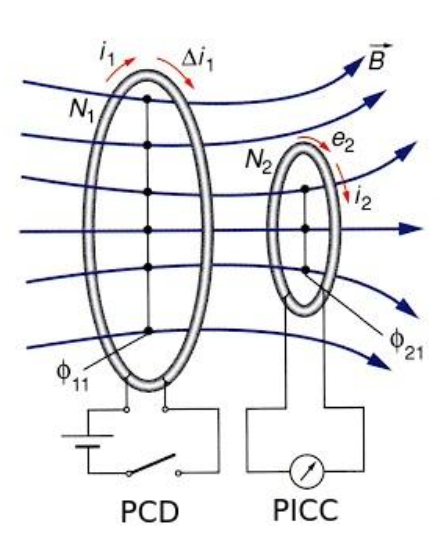
\includegraphics[scale=0.6]{antena/antena_trafo.png}
\caption{Densidad de flujo magnético generada por el PCD e inducida en la antena del PICC.}
\label{fig:trafo}
\end{figure}

La Figura \ref{fig:acople} muestra el factor de acoplamiento K frente al diámetro de antena D en base a la distancia de operación requerida de 10 cm.
Aunque la curva es muy plana en su parte superior, se puede ver que un diámetro de antena menos de 15 cm muestra una disminución significativa del factor de acoplamiento (y rendimiento). El factor de acoplamiento y el rendimiento disminuye drásticamente cuando el diámetro de la antena es inferior a 12 cm.

\begin{figure}[H]
\centering
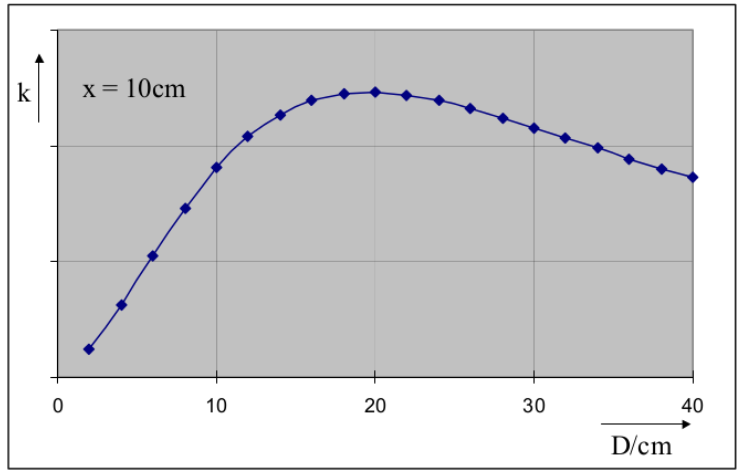
\includegraphics[scale=0.5]{antena/antena_acople.png}
\caption{Factor de acoplamiento vs Diámetro de la antena.}
\label{fig:acople}
\end{figure}

El inductor del PICC ($L_{PICC}$) está acoplado a la antena del transponder ($L_{PCD}$), existiendo así una inductancia mutua M entre ellos (Figura C). Esta inductancia mutua puede definirse en función de las inductancias de las antenas y el coeficiente de acoplamiento (k) como:
\begin{equation}
M = k \sqrt{L_{PCD}L_{PICC}}
\end{equation}

\begin{figure}[H]
\centering
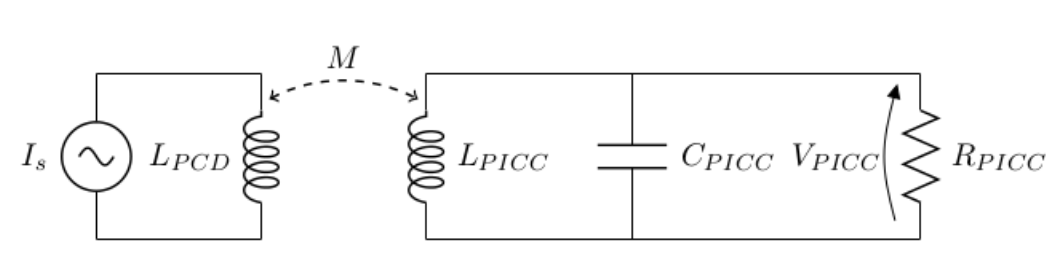
\includegraphics[scale=0.5]{antena/antena_m.png}
\caption{Modelo simplificado del acoplamiento inductivo entre el PCD y el PICC.}
\label{fig:acoplem}
\end{figure}

Cabe destacar que la relación mostrada anteriormente entre el tamaño de la antena y la distancia de operación es independiente del número de espiras (y la inductancia) de la antena PCD.
El coeficiente de acoplamiento es un factor limitante no sólo para la energía que se transporta al PICC, sino también para la respuesta del PICC que debe ser recibida por el PCD.


\subsection{Modelo de simulación}

En la nota de aplicación de Zheng Zhu \cite{shunt1}, se detalla el modelo de simulación para una antena HF RFID. El modelo se muestra en la figura \ref{fig:ant_model} y los valores de los componentes en la tabla \ref{table:sim_values}.

\begin{figure}[H]
\centering
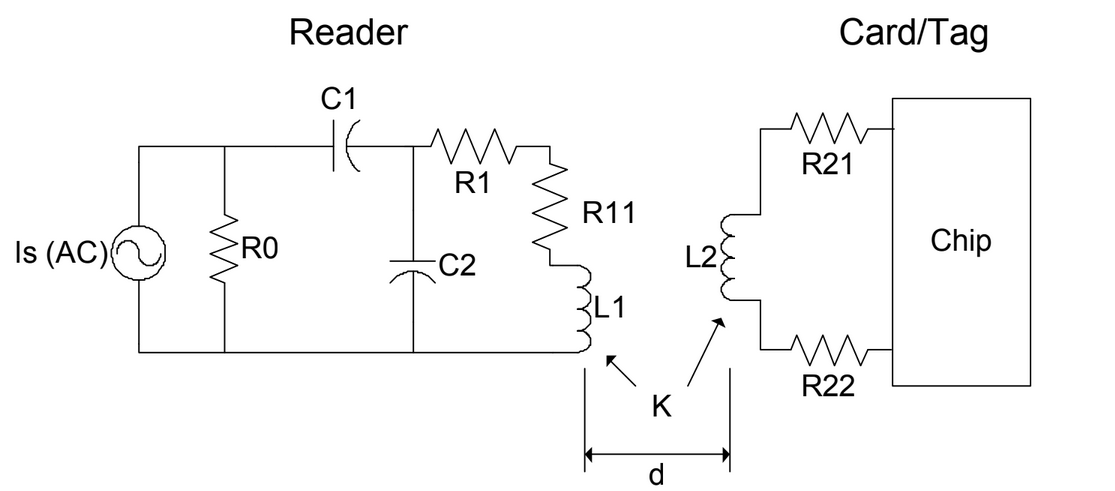
\includegraphics[width=0.9\linewidth]{antena/antena_model.png}
\caption{Modelo de simulación de una antena en HF}
\label{fig:ant_model}
\end{figure}

\begin{table}[h]
\centering
\caption{Valores de los componentes para el modelo de simulación}
\label{table:sim_values}
\begin{tabular}{c|c|c}
Componentes & Explicación                           & Valores típicos                      \\ \hline
Is          & Fuente de corriente ideal             & 162 mA efectivos (AC) para 13.56 MHz \\
R0          & Resistencia de la fuente de corriente & 50                                   \\
C1          & PCD circuito de matching              & 47 pF                                \\
C2          & PCD circuito de matching              & 184 pF                               \\
R1          & PCD circuito de matching              & 2                                    \\
R11         & Resistencia de la antena PCD          & 0.2                                  \\
L1          & Inductancia de la antena PCD          & 0.6 uH                               \\
L2          & Inductancia de la antena PICC         & 4.08 uH                              \\
R21, R22    & Resistencia de la antena PICC         & 1.32                                 \\
K           & Factor de acople                      & 0.008 (15 cm), 0.12 (0 cm)          
\end{tabular}
\end{table}

\clearpage



\clearpage
\section{Diseño de la Antena}
\label{sec:antena_dise}
\subsection{Introducción}
Esta sección contiene los conceptos básicos para el diseño de una antena de tipo solenoide,
para aplicaciones RFID.
A lo largo de la guía se dan ejemplos para el cálculo de una antena con las siguientes
características:
\begin{itemize}
\item Alambre de cobre de 0.3mm de diámetro.
\item Número de espiras N = 5.
\item 0,05 m de diámetro interior.
\end{itemize}

\begin{figure}[H]
\centering
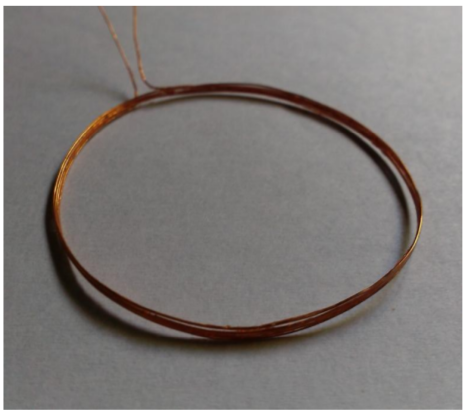
\includegraphics[scale=0.4]{antena/Antena.png}
\caption{Antena diseñada.}
\label{fig:antena}
\end{figure}

\subsection{Cálculo de la frecuencia de Resonancia}

\begin{figure}[H]
\centering
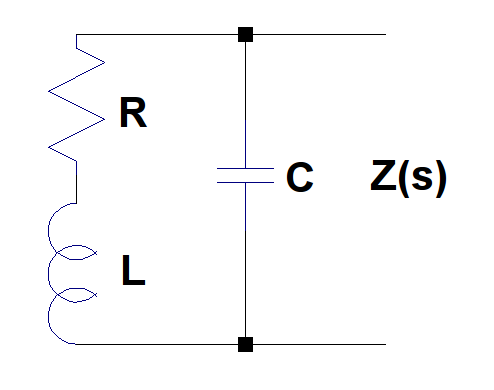
\includegraphics[scale=0.3]{antena/Antena_Equivalente.png}
\caption{Circuito de sintonía del PIC.}
\label{fig:antena_eq}
\end{figure}

El circuito muestra una impedancia:

\begin{equation}
Z(S) = \frac{LS + R}{LCS^2 + RCS + 1}
\end{equation}

Barriendo por el eje jω (S = jω) y multiplicando por el conjugado para separar la parte real
y la parte imaginaria:

$$Z(S)|_{S=j\omega} = \frac{j\omega L + R}{-LC\omega ^2 + j\omega RC + 1}$$
$$Z(S)|_{S=j\omega} = \frac{R + j\omega L}{(1 - LC\omega^2) + j\omega RC} * \frac{(1 - LC\omega ^2) - j(\omega RC)}{(1 - LC\omega ^2) - j(\omega)}$$
$$Z(j\omega) = \Omega + jX = \frac{R(1 - LC\omega ^2)-jR^2C\omega+j\omega L(1-LC\omega ^2)+\omega ^2 RLC}{(1 - LC\omega ^2)^2 - (RC\omega )^2}$$
$$Z(j\omega) = \Omega + jX = \frac{R(1 - LC\omega ^2)+\omega ^2RLC}{(1 - LC\omega ^2)^2 - (RC\omega )^2}+j\frac{\omega L(1 - LC\omega ^2)-R^2C\omega}{(1 - LC\omega ^2)^2 - (RC\omega )^2}$$

La frecuencia de resonancia se alcanza cuando la parte imaginaria de la impedancia se
hace nula, osea $X(j\omega _o) = 0$

$$X(j\omega _o) = \omega _o L(1 - LC\omega _o ^2)-R^2C\omega _o = 0$$
$$X(j\omega _o) = L(1 - LC\omega _o ^2)-R^2C = 0$$
\begin{equation}
\boxed{\omega _o = \sqrt[]{\frac{R ^2C - L}{L^2C}}}
\end{equation}

Para el diseño de una antena RFID, es necesario considerar el Q del inductor, ya que nos
interesa qué tan selectiva es la antena. Por definición $Q = \frac{\omega L}{R}$, siendo Q la selectividad del circuito resonante, \omega la frecuencia angular, L la inductancia y R la resistencia (pérdidas) de la antena.

\begin{figure}[H]
\centering
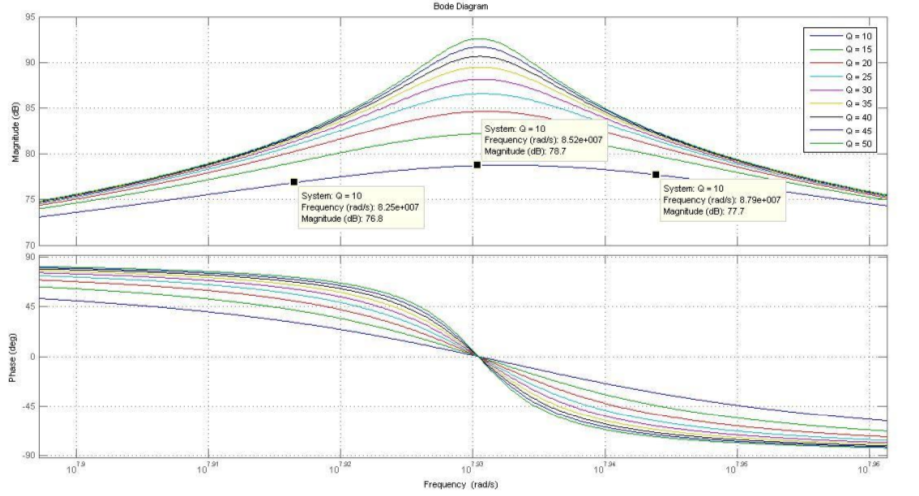
\includegraphics[scale=0.5]{antena/Respuesta_Frecuencia.png}
\caption{Respuesta en frecuencia del circuito de sintonía.}
\label{fig:transf_frec}
\end{figure}

Para la comunicación desde el PICC al PCD, se modula la portadora con ASK (modulación por desplazamiento de amplitud) a una frecuencia de 847 kHz. Esto nos produce, en el espectro, dos bandas laterales con respecto a la frecuencia central. En la figura \ref{fig:transf_frec} se ve que con un Q de 10, la respuesta cae aproximadamente 1 dB.
Si se aumenta el Q, el circuito se vuelve más selectivo, filtrando las bandas laterales y perdiendo así la modulación. 
Según \cite{antena_guide}, el factor de calidad debe ser:
\begin{equation}
\boxed{Q \leq \frac{f_c}{2B}}
\end{equation}
Siendo $f_c$ la frecuencia central (en este caso 13,56MHz) y B el ancho de banda. El Q
óptimo para la norma ISO 15693 es $9\leq Q\geq 16$.
Por lo tanto, para este diseño, se escoge un Q de 10.

\subsection{Tensión inducida en la bobina}
A partir de las leyes del magnetismo, se despeja la ecuación de la tensión inducida en una bobina:
\begin{equation}
V = -N\frac{d\phi}{dt}
\end{equation}
\begin{equation}
\phi = \int_{}^{}  B \, dS
\end{equation}
Suponiendo B, S y \psi constantes en el intervalo a analizar, se llega a la siguiente fórmula:
\begin{equation}
\boxed{V = 2 \pi fNBS\cos(\alpha)}
\end{equation}

Siendo f la frecuencia de trabajo, N el número de espiras, B la densidad de flujo magnético, S el área de la bobina y \alpha el ángulo comprendido entre el PICC y el PCD.\newline

\underline {Ejemplo:}\newline

$$f = 13.56 MHz ; \alpha = \frac{\pi}{2}$$
$$S = \pi (0.025m^2) = 1.96*10^{-3}$$
$$1.5 < H < 7 [\frac{A}{m}]$$


Entonces:
$$0.315*N < V < 1.469*N  [Volts]$$

Puede observarse que la tensión inducida en la bobina es directamente proporcional al número de espiras. Si N = 5, la tensión inducida estará comprendida, aproximadamente, entre 1.575 y 7.345 Volts.

\subsection{Resistencia en continua de la antena}
La resistencia depende del material y de su geometría. Es directamente proporcional a la
longitud e inversamente proporcional a la sección:
\begin{equation}
\boxed{R_{DC} = \rho \frac{l}{S}}
\end{equation}
Siendo \rho la resistividad del material, l la longitud y S la sección.\newline

\underline {Ejemplo:}\newline

Se desea calcular la resistencia en continua de una bobina de cobre. La bobina tiene un
diámetro de 0,05m, y la sección del cable es 0,3mm.

$$ R_{DC} = \rho _{cu}\frac{l}{S} $$
$$ R_{DC} = \frac{0.017 \Omega mm^2}{m}\frac{N 0.05m \pi}{\pi (0.15mm)^2} $$
$$ R_{DC} = 0.03\wideparen{7} N \Omega $$
Para un N igual a 5:
$$ R_{DC} = 0.1\wideparen{8} \Omega $$

\subsection{Resistencia en alterna de la bobina}
En altas frecuencias, la densidad de corriente es más alta en la superficie del conductor y
más baja en el centro. Este efecto se llama profundidad de penetración \delta.
Según  \cite{antena_AN710}, la resistencia puede aproximarse sabiendo el radio del conductor y la profundidad de penetración.
La profundidad de penetración es:

\begin{equation}
\boxed{\delta = \frac{1}{\sqrt[]{\pi f \mu \sigma }}}
\end{equation}

Siendo f la frecuencia, \mu la permeabilidad del material y \sigma la conductividad.
Para un alambre de cobre, trabajando a una frecuencia de 13.56MHz, la profundidad de
penetración es 0.018 mm.
La resistencia en alterna es, entonces:

\begin{equation}
\boxed{R_{ac} = R_{DC} \frac{a}{1\delta}}
\end{equation}
Siendo $R_{DC}$ la resistencia en continua, y 'a' el radio del conductor.

Siguiendo el ejemplo anterior, se tiene:

$$ R_{ac} = 0.18 \frac{0.15}{2*0.018} \Omega = 0.75 \Omega $$

\subsection{Inductancia de una bobina de N espiras}

\begin{figure}[H]
\centering
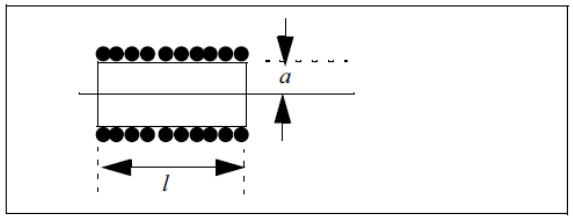
\includegraphics[scale=0.5]{antena/Bobina_N_Espiras.png}
\caption{Geometría de una bobina de N espiras.}
\label{fig:N_esp}
\end{figure}

La inductancia de una bobina depende, principalmente, de la geometría y el número de
espiras.

Según \cite{antena_AN710}, para calcular la inductancia L:

\begin{equation}
\boxed{L = \frac{(aN)^2}{22.9 a+25.4 l}}
\end{equation}

Donde a es el radio de la bobina, l es el largo, y N el número de espiras.\newline

\underline {Ejemplo:}\newline

Se desea calcular la inductancia de una bobina con las siguientes especificaciones.

\begin{itemize}
\item a = 25mm
\item l = 0.3mm N
\item N = 5
\end{itemize}

$$ L = \frac{(25mm*5)^2}{22.9*25mm+25.4*0.3mm*5}\mu Hy = 25.59 \mu Hy$$

\subsection{Cálculo del factor de calidad o selectividad Q}
El factor de calidad se calcula como:

\begin{equation}
\boxed{Q =\frac{\omega L}{R_{ac}}}
\end{equation}
\newline
\underline{Ejemplo:}\newline
Para los valores de L y R calculados anteriormente, hallar Q.

\begin{itemize}
\item L = 25.59 \mu Hy
\item $R_{ac}$ = 0.75 \Omega
\item \omega = 2\pi *13.56MHz
\end{itemize}

$$ Q = \frac{2\pi *13.56MHz*25.59\mu Hy}{0.75 \Omega} = 1907 $$

\subsubsection{Mediciones del solenoide de 5 espiras}
Se fabricó una antena con las características mencionadas al principio de la guía, y se midió
con un medidor RLC (Tonghui TH2826A). Luego se contrastaron los valores con un Qmetro
analógico.

\begin{figure}[H]
\centering
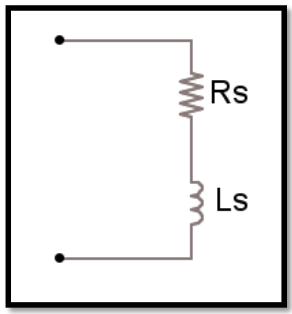
\includegraphics[scale=0.5]{antena/Equivalente_Bobina_Serie.png}
\caption{Circuito equivalente del inductor real.}
\label{fig:L_real}
\end{figure}


Se obtuvieron los siguientes datos:

\begin{table}[H]
\centering
\caption{Mediciones de la Antena}
\label{table:med_antena}
\begin{tabular}{c|c|c|c}
\textbf{Frecuencia [Hz]} & \textbf{Ls [Hy]}       & \textbf{Rs [\Omega]} & \textbf{Q}                                                                                \\ \hline
1000                    & 2.9039E-06 & 0.2648   & 0.06890291                                                                             \\
2000                 & 3.3124E-06 & 0.278   & 0.14972785                                                                             \\
100000                  & 3.2564E-06 & 0.2776   & 7.37061094                                                                                 \\
200000                  & 3.2404E-06 & 0.3012   & 13.5193621                                                                             \\
500000                  & 3.2262E-06 & 0.374   & 27.0998486                                                                             \\
800000                  & 3.1978E-06 & 0.4432   & 36.2680427                                                                             \\
1000000                  & 3.1899E-06 & 0.4705   & 42.598928                                                                             \\
200000                  & 3.0715E-06 & 0.7688   & 50.2041871          
\end{tabular}
\end{table}

\begin{figure}[H]
\centering
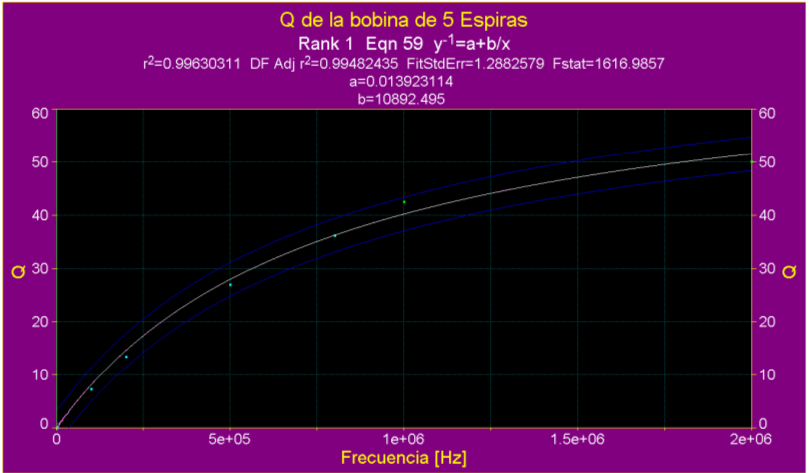
\includegraphics[scale=0.5]{antena/Simulacion_Q_Antena.png}
\caption{Variación del Q de la bobina con la frecuencia.}
\label{fig:L_Qsim}
\end{figure}

Ajustando la curva, vemos que la Q varía aproximadamente de la siguiente forma:

$$ Q = \frac{1}{a + \frac{b}{f}} = \frac{1}{0.0139 + \frac{10892.495}{f}} $$

Para la frecuencia de interés (f = 13.56 MHz):
$$Q = 67.90528 \pm 3.152254 \textrm{      ;con un intervalo de confianza del 95\%} $$ 

\subsection{Antena para testing}
Tomándose como base las normas de testeo ISO/IEC10373 \cite{nfc_test} se realizó la fabricación de una antena para las pruebas de laboratorio del circuito integrado \ref{fig:L_test}.
La inductancia mostrada por esta antena fue
de 1,6 μHy, obteniendo, para una resonancia a
13,56 MHz, una capacidad paralela necesaria de
88 pF.



\begin{figure}[H]
\centering
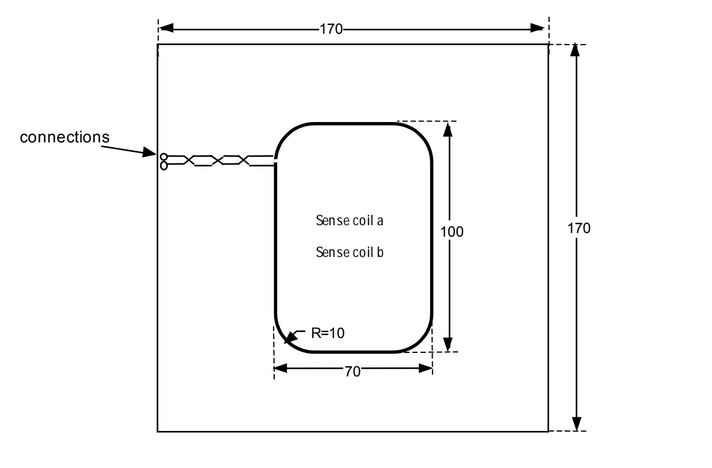
\includegraphics[scale=0.6]{antena/Bobina_Testing.JPG}
\caption{Antena para testing (ISO/IEC10373).}
\label{fig:L_test}
\end{figure}






\clearpage
\section{Diseño del Front-End analógico}
\label{sec:analog}
En esta sección se describe el diseño completo del Front-End analógico compatible con la norma ISO/IEC 14443A. En la próxima sección se verán los resultados y mediciones del diseño. 

\subsection{Diseño de un CI}
El diseño de circuitos integrados se mantiene
siempre dentro de cierto número de pasos que
no varían con el circuito. Estos pasos pueden
detallarse en los ítems que se muestran a continuación \cite{detect_fallas_500nm}.

\begin{enumerate}
\item Diseño teórico: definición del comportamiento
deseado y elección de la topología del circuito.
\item Descripción del comportamiento: iteración de
simulaciones y modificaciones hasta la obtención
del comportamiento deseado.
\item Layout: realización, en el software especializado
(Synopsys Custom Designer en nuestro
desarrollo), del diseño físico en silicio del
circuito, a partir de las reglas de diseño de la
tecnología.
\item Design Rules Check (DRC), Layout vs. Schematic
(LVS) y Parasitic Extraction (PEX): análisis
correspondientes a la verificación del diseño.
En esta etapa se realiza la búsqueda, en
el layout, de violaciones a las reglas de diseño
(DRC). Luego, se verifica que el layout y el esquemático
diseñados correspondan el uno con
el otro (LVS). Al final, se realiza una simulación
teniendo en cuenta los componentes parásitos
que aparecen en el diseño físico (PEX). Las herramientas
utilizadas para esto son Mentor Graphics y Synopsys.
\item Iteración en el diseño: si en el transcurrir de
alguno de los pasos no se cumple con el comportamiento
estipulado del diseño, se retorna al
ítem número 2 y se vuelven a realizar los pasos
posteriores hasta encontrar el comportamiento
deseado y detallado en el ítem 1.
\end{enumerate}

\subsection{Descripción general de funcionamiento}

\begin{figure}[H]
\centering
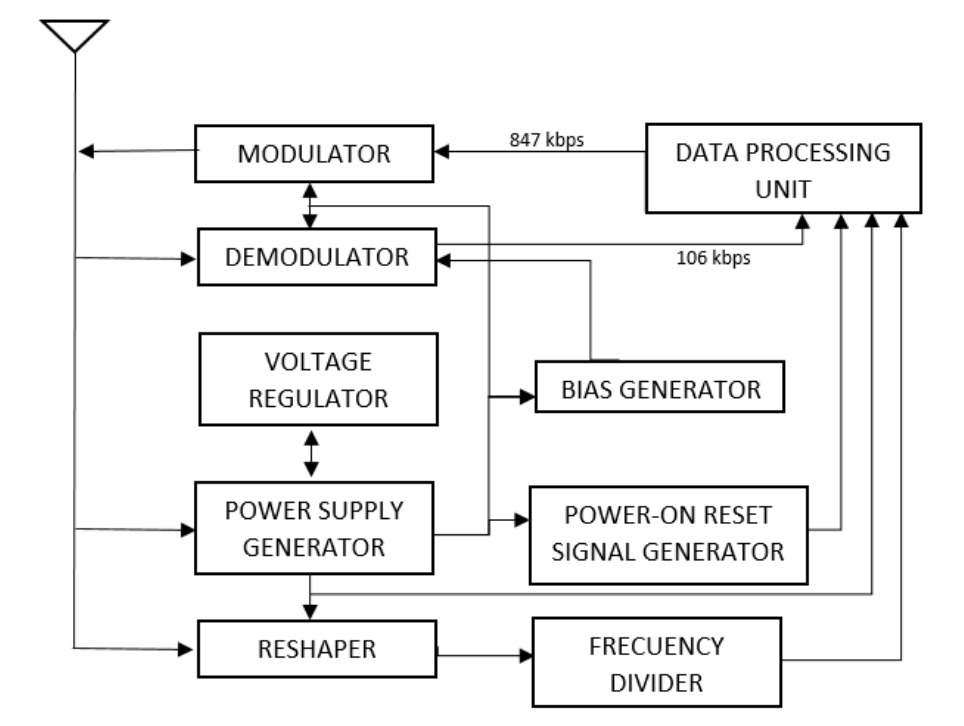
\includegraphics[scale=0.4]{modulos_rfid.png}
\caption{Módulos Front-End Analógico}
\label{fig:modulos_rfid}
\end{figure}

La tarjeta de contacto consiste en dos secciones principales: Sección de RF (Front-End Analógico) y la Unidad de Procesamiento de Datos (DPU). Los módulos del Front-End Analógico (AFE) se muestra en la figura \ref{fig:modulos_rfid}, el cuál consiste en un generador de tensión \textit{(Power Supply Generator - PSG)}, un generador de clock \textit{(Clock Generator - CG)}, un regulador de tensión continua \textit{(Voltage Regulator - VR)}, un \textit{Power On Reset (POR)}, un modulador y un demodulador.

El principio de funcionamiento es lo siguiente: 

\begin{itemize}
\item Cuando el PICC (tag) entra a un campo electromagnético, osea, cuando se acerca al PCD (lector), induce una tensión en la antena del PICC y energiza el módulo PSG. 
\item PSG contiene un rectificador de tensión alterna y un regulador Shunt (Figura \ref{fig:modulos_picc}). Éste módulo tiene como propósito entregar una tensión continua a la salida y limitar la tensión máxima de operación que puede soportar el chip. La salida limitada en tensión va conectado a la entrada de VG. 
\item VG regula la entrada y provee una tensión constante a la salida de la misma. Éste módulo es muy importante ya que alimenta a todo el chip. 
\item El POR entrega un cero lógico por un tiempo determinado al recibir la alimentación de VG. Ésto sirve para resetear todos los flip flops de la DPU. 
\item El modulador y demodulador son módulos analógicos que sirven para que el PCD se pueda comunicar con el PICC.
\end{itemize}

\begin{figure}[H]
\centering
\includegraphics[scale=0.5]{picc.png}
\caption{Módulos PICC (Power Management)}
\label{fig:modulos_picc}
\end{figure}

A continuación se describe detalladamente el funcionamiento de cada módulo del AFE.


\subsection{Generador de Tensión (PSG)}

El PSG se divide en dos partes: rectificación de la fuente de alterna (13,56 MHz) y límitación de potencia. 

La primera parte cumple la función de rectificar el campo magnético inducido desde el lector. Se implementó un rectificador con transistores NMOS funcionando como diodo. En la figura \ref{fig:rectifier} se puede ver la topología implementada. 

\begin{figure}[H]
\centering
\includegraphics[scale=0.6]{circuitos/Rectifier.png}
\caption{Rectificador de onda completa con transistores NMOS}
\label{fig:rectifier}
\end{figure}

Cabe destacar que la caída de tensión sobre el rectificador depende inversamente con el ancho de canal (W) del MOS. Mientras más ancho es W, menos tensión cae en esta etapa. Es lógico que el limitante en éste caso es el área. 

La segunda parte cumple la función de proteger el chip, ya que para que el chip sea compatible con la norma ISO/IEC 14443-2, el PICC debe ser capaz de funcionar para distintas intensidades de campo magnético (1,5-7,5 A/m rms). En la figura \ref{fig:shunt} se muestra la topología.

\begin{figure}[H]
\centering
\includegraphics[scale=0.045]{circuitos/Shunt.png}
\caption{Limitador de potencia - Shunt}
\label{fig:shunt}
\end{figure}

El limitador shunt tiene como característica prender el transistor Q9 al superar una tensión de umbral en los bornes del módulo, osea que, éste transistor trabaja idealmente sólo en corte y saturación. 

Como las dos tecnologías que se utilizó tienen distintas tensiones de operación (3,3 a 5 V para ONC5 y 1,2 a 2,5 V para GF130), las tensiones de umbral varían. En las figuras \ref{fig:shunt_500} y \ref{fig:shunt_130} se muestran las tensiones de umbral para cada tecnología. Como se puede observar, para ONC5 el circuito se prende en 4,5 V y para GF130 se prende en 2,8 V.

Entre el rectificador y el shunt se encuentra un capacitor de aproximadamente 400 pF, éste capacitor depende de la tensión de operación de la tecnología y del proceso. 

\begin{figure}[H]
\centering
\includegraphics[width=0.9\linewidth]{simulaciones/shunt_500.png}
\caption{Tension de umbral (ONC5)}
\label{fig:shunt_500}
\end{figure}

\begin{figure}[H]
\centering
\includegraphics[width=0.9\linewidth]{simulaciones/shunt_130.png}
\caption{Tension de umbral (GF130)}
\label{fig:shunt_130}
\end{figure}


\subsection{Generador de clock (CG)}

El generador de clock obtiene el reloj a partir de la antena, ya que el lector emite una frecuencia de 13,56 MHz +- 7 kHz, que está especificado en la norma ISO/IEC 14443-2 \ref{sec:iso}. El módulo (figura \ref{fig:clock_gen}) consiste principalmente en dos Flip Flop tipo D (que actúa como divisor de clock por 2) y una compuerta XOR.

Básicamente funciona de la siguiente manera: Aprovechando la diferencia de fase entre los bornes de la antena con respecto a masa (180 grados de diferencia de fase), se le hace pasar por los flip flop D y la XOR para recuperar el clock (figura \ref{fig:clock_gen_sim}).

\begin{figure}[H]
\centering
\includegraphics[width=0.5\linewidth]{circuitos/CLK.png}
\caption{Generador de clock}
\label{fig:clock_gen}
\end{figure}

\begin{figure}[H]
\centering
\includegraphics[width=0.9\linewidth]{circuitos/clk_sim.png}
\caption{Generador de clock (Simulación)}
\label{fig:clock_gen_sim}
\end{figure}

\subsection{Regulador de Voltaje (VR)}

El regulador de voltaje regula la tensión proveniente del PSG y provee una tensión continua constante a la salida del módulo. Éste módulo funciona como alimentación para los demás módulos del chip. La topología de la VR se puede ver en la figura \ref{fig:ldo}. Éste módulo consiste principalmente en 3 partes: Un amplificador operacional (OP-AMP) que es usado como amplificador de error (Actúa como regulación, amplifica la diferencia entre una tensión de referencia conocida con respecto a la tensión de salida); un transistor serie a la salida que es usado como amplificador de corriente; R3 y R4 son usados como divisor de voltaje resistivo (Ecuación \ref{eq:vref}).  

\begin{figure}[H]
\centering
\includegraphics[width=0.5\linewidth]{circuitos/LDO.png}
\caption{Regulador de Voltage}
\label{fig:ldo}
\end{figure}

\begin{equation} \label{eq:vref}
VDD = Vref*(1+R3/R4)
\end{equation}

\subsection{Modulador}

El modulador cambia la impedancia que vista desde la PCD. Existen dos tipos de modulación: modulación resistiva y capacitiva. Ambos tipos crean una subportadora cerca de 13.56MHz. Se adoptó la modulación resistiva para éste diseño. La topología se muestra en la figura \ref{fig:mod}. Para más información, ver la sección \ref{subsec:modulador}.

\begin{figure}[H]
\centering
\includegraphics[width=0.3\linewidth]{circuitos/MOD.png}
\caption{Modulador}
\label{fig:mod}
\end{figure}

\subsection{Demodulador}

El demodulador recupera la trama digital transmitido por el PCD. Para el tag tipo A, se extraen los datos con un detector de envolvente. La salida del detector de envolve se conecta a un buffer. La topología se muestra en la figura \ref{fig:demod}. Para más información, ver sección \ref{subsec:demodulador}.

\begin{figure}[H]
\centering
\includegraphics[width=0.7\linewidth]{circuitos/DEM.png}
\caption{Demodulador}
\label{fig:demod}
\end{figure}

\subsection{Power On Reset (POR)}

Éste módulo es usado para resetear la máquina digital (\textit{NFC Digital Core}) cuando se acerca la PICC a la PCD. La POR consiste principalmente en un filtro pasabajos RC y un buffer. El esquemático se muestra en la figura \ref{fig:por}.

\begin{figure}[H]
\caption{Power on Reset}
\label{fig:por}
\includegraphics[width=0.3\linewidth]{circuitos/POR.png}
\centering
\end{figure}

\subsection{Diseño final}

Los valores de los componentes que se utilizó para el diseño y fabricación del proceso GF130 se puede ver en las tablas \ref{table:trans_specs_130} y \ref{table:res_specs_130}. Y los valores para el proceso ONC5 se encuentran en las tablas \ref{table:trans_specs_500} y \ref{table:res_specs_500}.


\begin{table}[H]
\centering
\begin{tabular}{c|c|c|c|c}
\textbf{Tipo}  		 & \textbf{Simbolo}	& \textbf{W}  & \textbf{L}  & \textbf{Fingers/Multiplicidad}  \\ \hline
NMOS                 & Q1,Q2,Q3,Q4    	& 10 um       & 0.4 um      & 20                \\
PMOS                 & Q5,Q6,Q7       	& 5 um        & 0.4 um      & 1                 \\
NMOS                 & Q8             	& 5 um        & 0.4 um      & 2                 \\
PMOS                 & Q9             	& 15 um       & 0.4 um      & 25                \\
PMOS                 & Q10,Q11        	& 1 um        & 3 um        & 2                 \\
NMOS                 & Q12,Q13        	& 2 um        & 1 um        & 2                 \\
NMOS                 & Q14            	& 0.5 um      & 3 um        & 1                 \\
PMOS                 & Q15            	& 10 um       & 0.4 um      & 10                \\
NMOS                 & Q16,Q17        	& 5 um        & 0.4 um      & 1                 \\
NMOS                 & Q18,Q19        	& 3 um        & 0.4 um      & 10                \\
\end{tabular}
\caption{Transistores GF130}
\label{table:trans_specs_130}
\end{table}

\begin{table}[H]
\centering
\begin{tabular}{c|c}
\textbf{Simbolos} 	&	\textbf{Valores} \\ \hline
R1              	& 10 k           \\
R2              	& 48.5 k         \\
R3,R4           	& 343 k          \\
R5,R6           	& 37.5 k         \\
R7,R8           	& 370            \\
R9              	& 150 k           \\
C1              	& 5p             \\
C2              	& 3.5 p          \\
C3              	& 7.8 p          \\
\end{tabular}
\caption{Componentes Adicionales GF130}
\label{table:res_specs_130}
\end{table}

\begin{table}[H]
\centering
\begin{tabular}{c|c|c|c|c}
\textbf{Tipo}  		 & \textbf{Simbolo}	& \textbf{W}  & \textbf{L}  & \textbf{Fingers/Multiplicidad}  \\ \hline
NMOS                 & Q1,Q2,Q3,Q4    	& 10 um       & 0.6 um      & 10                \\
PMOS                 & Q5,Q6,Q7,Q7bis   & 5 um        & 0.6 um      & 5                 \\
NMOS                 & Q8             	& 5 um        & 0.6 um      & 5                 \\
PMOS                 & Q9             	& 10 um       & 0.6 um      & 15                \\
PMOS                 & Q10,Q11        	& 12 um       & 3 um        & 1                 \\
NMOS                 & Q12,Q13        	& 3 um        & 3 um        & 1                 \\
NMOS                 & Q14            	& 1 um        & 3 um        & 1                 \\
PMOS                 & Q15            	& 10 um       & 0.6 um      & 20                \\
NMOS                 & Q16,Q17        	& 5 um        & 0.6 um      & 4                 \\
NMOS                 & Q18,Q19        	& 15 um       & 0.6 um      & 10                \\
\end{tabular}
\caption{Transistores ONC5}
\label{table:trans_specs_500}
\end{table}

\begin{table}[H]
\centering
\begin{tabular}{c|c}
\textbf{Simbolos} 	&	\textbf{Valores} \\ \hline
R1              	& 50 k           \\
R2              	& 20 k           \\
R3           	    & 280 k          \\
R4           	    & 210 k          \\
R5,R6           	& 0, 6 k         \\
R7,R8           	& 136.5          \\
R9              	& 583 k          \\
C1              	& 3.48 p         \\
C2              	& 0.336 p        \\
C3              	& 1.44 p        \\

\end{tabular}
\caption{Componentes Adicionales ONC5}
\label{table:res_specs_500}
\end{table}

El layout final del Front-end analógico (AFE) se muestran en las Figuras \ref{fig:onc5} y \ref{fig:gf130}. Fueron diseñados para los procesos On Semiconductor 500 nm (ONC5) y Global Foundries 130 nm (GF130) mencionados anteriormente. 

Para el proceso ONC5, el AFE ocupa un área de 0,7 x 0,4 mm; Mientras que para el proceso GF130, solamente 0,3 x 0,2 mm. 

\begin{figure}[H]

\subfloat[Proceso ONC5]{\label{fig:onc5}\includegraphics[width=0.5\linewidth]{circuitos/onc5_layout.png}}
\subfloat[Proceso GF130]{\label{fig:gf130}\includegraphics[width=0.5\linewidth]{circuitos/gf130_layout.png}}

\caption{Layout del Front-End Analógico}
\label{fig:layout_completo}
\end{figure}




\clearpage
\section{Diseño del detector de símbolos}
\label{sec:digital}
El detector de símbolos necesario para lograr una prueba de funcionamiento de los circuitos integrados compuestos por el front-end analógico de un sistema RFID, se desarrolló mediante el lenguaje de descripción de hardware (HDL) Verilog.

\subsection{Características de la comunicación}

\subsubsection{Frames}
La ISO/IEC14443 tipo A agrupa los bits de datos en un frame con un comienzo de frame (SoF), un fin de frame (EoF) y un bit de paridad (P) al final de cada byte de datos (8 bits de datos), excepto para frames cortos. El EoF solo se usa para la comunicación desde el PCD a PICC.

\begin{figure}[H]
\centering
\includegraphics[scale=0.5]{digital/Frame_TipoA.png}
\caption{Formato de frame de Tipo A.}
\label{fig:frame_A}
\end{figure}

\subsubsection{Codificaciones}
Debido a la dificultad para determinar la diferencia entre un bit cero y el transmisor realmente desconectado, los datos necesita algunas reglas adicionales, es decir, debe codificarse. Los métodos de codificación utilizados en esta especificación son:

\begin{itemize}
\item Manchester \ref{fig:coding_A}.
\item Miller modificado \ref{fig:coding_A}.
\end{itemize}

\begin{figure}[H]
\centering
\includegraphics[scale=0.5]{digital/Codificaciones.png}
\caption{Codificaciones utilizadas.}
\label{fig:coding_A}
\end{figure}

En la Tipo A se utiliza la codificación Manchester para la comunicación del PICC hacia el PCD y Miller Modificado para la del PCD hacia el PICC.

\subsubsection{Bit Rate}
El tiempo de una señal digital se indica por medio de unidades de tiempo elementales (etu).
Para esta especificación, un etu equivale a un período de un bit, es decir, el tiempo para transmitir una unidad de información.\newline
Para la comunicación PCD -> PICC:
$$ 1 etu =  \frac{128}{f_c D_{PCD->PICC}}$$\newline
Para la comunicación PICC -> PCD:
$$ 1 etu =  \frac{8}{f_s D_{PICC->PCD}}$$
Donde $f_c$ es la frecuencia de portadora generada por el PCD, $f_s$ la frecuencia de subportadora generada por el PICC. El valor inicial de los dividores $D_{PCD->PICC}$ y $D_{PICC->PCD}$ es 1, lo que da una velocidad de bit inicial de 106kb/s.
Entonces, durante este documento, se hablará de una velocidad de bit de $f_c$/128 \~ 106kbit/s en ambas direcciones de la comunicación.


\subsubsection{Sincronización}
A diferencia de la Tipo B, la Tipo A no tiene una secuencia de sincronización. Para la comunicación desde el PCD al PICC, la Tipo A usa 100\% ASK. El nivel inferior es un disparador suficiente para iniciar la demodulación e indicar el inicio del primer símbolo.
Para la comunicación PICC a PCD, la comunicación es síncrona y alineada a la cuadrícula. El inicio de una secuencia se determina contando el número de ciclos de la portadora transcurridos desde el último nivel inferior del comando.

\subsubsection{Codificación de bits}
Aquí se especifica cómo son los valores lógicos para la norma ISO/IEC14443 Tipo A.

La codificación utilizada por el PCD es Miller Modificado con modulación ASK 100\% (Fig. \ref{fig:Mil}).

\begin{figure}[H]
\centering
\includegraphics[scale=0.5]{digital/Miller_Modif.png}
\caption{Miller modificado con modulación ASK al 100\%.}
\label{fig:Mil}
\end{figure}

Los símbolos definidos son los siguientes:
\begin{itemize}
\item Símbolo X: nivel bajo luego de la mitad de la duración del bit.
\item Símbolo Y: toda la duración del bit sin modulación.
\item Símbolo Z: el comienzo del bit en nivel bajo.
\end{itemize}

La codificación utilizada por el PICC es Manchester con modulación OOK con subportadora (Fig. \ref{fig:Man}).

\begin{figure}[H]
\centering
\includegraphics[scale=0.5]{digital/Manchester.png}
\caption{Codificación manchester con modulación OOK.}
\label{fig:Man}
\end{figure}

Los símbolos definidos son los siguientes:
\begin{itemize}
\item Símbolo D: la portadora es modulada por la subportadora durante la primer parte del bit.
\item Símbolo E: la portadora es modulada por la subportadora durante la segunda parte del bit.
\item Símbolo F: la portadora no es modulada por la subportadora durante toda la duración del bit.
\end{itemize}

\subsubsection{Desincronización}
Consiste en una violación de las reglas normales de codificación/decodificación para un "0" lógico y un "1" lógico.


\subsubsection{Formato de frame}
En esta sección se definen los frames utilizados en la norma tipo A. 
Ésta utiliza dos tipos de frames:
\begin{itemize}
\item Frame corto.\\
El frame corto es utilizado para comenzar la comunicación y consiste en lo siguiente (Fig.\ref{fig:short_frame}):\\
- SoF ( Inicio de trama - Start of frame ).\\
- 7 bit de información transmitidos primero los LBS.\\
- EoF ( Fin de trama - End of Frame ).\\
No se añade paridad.
\end{itemize}

\begin{figure}[H]
\centering
\includegraphics[scale=0.5]{digital/Short_Frame.png}
\caption{Frame corto.}
\label{fig:short_frame}
\end{figure}

\begin{itemize}
\item Frame standar.\\
 El frame standar para el intercambio de información y consiste en lo siguiente (Fig\ref{fig:standar_frame}).\\
 - SoF.\\
 - n x (8 bits de información + bit de paridad impar), con n \geq  1.\\
 - EoF (sólo desde el PCD al PICC).
\end{itemize}

\begin{figure}[H]
\centering
\includegraphics[scale=0.5]{digital/Standar_Frame.png}
\caption{Frame standar.}
\label{fig:standar_frame}
\end{figure}

Para la comunicación desde el PCD al PICC, el SoF debe ser un "0" lógico.
Para la comunicación desde el PICC al PCD, el SoF debe ser un "1" lógico.
Para la comunicación PCD a PICC, un frame debe terminar con EoF.
Este EoF debe ser un "0" lógico.

\subsubsection{Tamaños de frame}
\begin{itemize}
\item FSD (Tamaño de frame para el PCD).\\
El FSD define el tamaño máximo de un frame que el PCD es capaz de recibir. El FSD es expresado en número de bytes de datos incluidos en el frame.\\ 
Para el Tipo A, el PCD
indica el FSD al PICC por el parámetro FSDI con el comando RATS 
\item FSC (Tamaño de frame para el PICC).\\
El FSC define el tamaño máximo de un frame aceptado por el PICC. El FSC es expresado en número de bytes de datos incluidos en el frame.\\ 
Para el tipo A, el PICC
indica el FSC a PCD por medio del FSCI en T0 del comando ATS.
\end{itemize}


\subsubsection{Set de comandos}

\begin{table}[H]
\centering
\begin{tabular}{c|c|c|c}
\textbf{Comando PCD} & \textbf{Respuesta PICC}                                                   \\ \hline
WUPA                    & ATQA                                                                        \\
REQA                 	& ATQA                                                                         \\
ANTICOLLISION CL1                  & UID CL1                                                                             \\
ANTICOLLISION CL2                  & UID CL2                                                                            \\
ANTICOLLISION CL3                 & UID CL3                                                                             \\
SELECT CL1                  & SAK                                                                            \\
SELECT CL2                  & SAK                                                                          \\
SELECT CL3                  & SAK                                                                                 \\
HLTA                  & -                                                                           \\
RATS                  & ATS       
\end{tabular}
\caption{Set de comandos}
\label{table:set_com}
\end{table}

\subsection{Estructura general del detector}
En la figura \ref{fig:dig_diag} se observa la estructura del detector de símbolos realizado.
Este detector consta de dos etapas de "traducción" de datos: un decodificador para convertir la información codificada por el PCD con Miller Modificado y un codificador para convertir la información generada por el PICC con codificación NRZ-L a codificación Manchester. Además, 

\begin{figure}[H]
\centering
\includegraphics[scale=0.3]{digital/Diagrama_Digi.png}
\caption{Diagrama básico del detector de símbolos.}
\label{fig:dig_diag}
\end{figure}

\subsection{Codificador}
Como ya se mencionó y, además, como puede observarse en la figura \ref{fig:dig_diag}, el codificador es el encargado de tomar los datos que genera la máquina de estado en NRZ-L y convertirlos en codificación Manchester para que ingresen al modulador de carga, transmitiendo, así, el mensaje desde el PICC al PCD.
El módulo responde a lo visto en la figura \ref{fig:Man}:
\begin{itemize}
\item Modula la portadora con la subportadora durante la primer mitad del bit cuando a su entrada llega un "1" lógico.
\item Modula la portadora con la subportadora durante la segunda mitad del bit cuando a su entrada llega un "0" lógico.
\end{itemize}
En la imagen \ref{fig:manch_code} se observa el módulo descripto mediante el lenguaje Verilog.

\begin{figure}[H]
\centering
\includegraphics[scale=0.45]{digital/Manchester_code.png}
\caption{Codificador Manchester en Verilog.}
\label{fig:manch_code}
\end{figure}

Durante el desarrollo de los módulos digitales del proyecto, se utilizó el "Icarus Verilog", una herramienta de compilación, síntesis y simulación de Verilog (IEEE-1364). Además del compilador mencionado, se usó el software para visualización de señales "GtkWave".
En la figura \ref{fig:manch_test} se muestra el resultado del testbench del módulo codificador con el GtkWave como herramienta de visualización de señales.

\begin{figure}[H]
\centering
\includegraphics[scale=0.5]{digital/Manchester_testbench.png}
\caption{Testbench del codificador Manchester.}
\label{fig:manch_test}
\end{figure}

En la etapa en la que el PICC debe comunicarse con el PCD, siempre habrá portadora, por esto es que se observa una señal de clock constante. Cada módulo contiene tanto un PoR (Power on Reset) que activa toda la lógica cuando el chip se energiza y una señal de habilitación (in\_ enable) que forma parte de la lógica de habilitación y desabilitación de los módulos durante la comunicación.
Una vez que la señal de habilitación se encuentra en estado alto, puede observarse que el codificador comienza a trabajar.

\subsection{Decodificador}

El módulo decodificador recibe las señales enviadas en codificación Miller Modificado por el PCD y demoduladas en el PICC para convertirlas a codificación NRZ-L, lo cuál ingresará a la máquina de estados como bits, puramente, en nivel alto ("1" lógicos) y bits, puramente, en nivel bajo ("0" lógicos). El conexionado de estas etapas puede observarse en la figura \ref{fig:dig_diag}.
En este caso, a diferencia del caso del codificador mencionado antes, la señal de clock, no es constante. Esto trae como necesidad la adición de un detector de pausa dentro del mismo decodificador, ya que al no tener clock, la lógica secuencial se ve afectada. Tanto el clock discontínuo (in\_ clock), como la señal del detector de pausa (in\_ pause) y las respectivas entradas y salidad de datos pueden observarse en la figura \ref{fig:mill_test}.

\begin{figure}[H]
\centering
\includegraphics[scale=0.5]{digital/Miller_testbench.png}
\caption{Testbench del decodificador Miller Modificado.}
\label{fig:mill_test}
\end{figure}

\subsection{Detección de los símbolos}
Los datos de salida del módulo decodificador ingresan en codificación NRZ-L a la máquina de estados. Esta máquina funciona siguiendo la lógica mostrada en la sección sobre la "Clasificación y estandarización de los sistemas RFID" donde se muestra en detalle lo normalizado por la norma ISO/IEC 14443 Tipo A.
En el desarrollo, se llevó a cabo la detección del comando REQA enviado por el PDC, respondiendo, una vez detectado, el comando ATQA. Puede observarse el resultado, obtenido en el banco de prueba, en la sección \ref{sec:resmedver}.


%\clearpage
%\section{Desarrollo de la solución a implementar}
%\label{sec:solucion}

\clearpage
\section{Resultados, Mediciones y Verificación}
\label{sec:resmedver}
Se mandó a fabricar los chips diseñados para los procesos ONC5 y GF130, en la figura \ref{fig:chip_completo} se muestra los chips con un microscopio electrónico.

\begin{figure}[H]
\subfloat[Chip proceso ONC5]{\label{fig:chip_onc5}\includegraphics[width=0.5\linewidth]{chip_500.png}}
\subfloat[Chip proceso GF130]{\label{fig:chip_gf130}\includegraphics[width=0.5\linewidth]{chip_130.png}}
\caption{Layout del Front-End Analógico}
\label{fig:chip_completo}
\end{figure}

Para validar y verificar los diseños, todos los módulos son testeados y comparados con resultados de simulación. La antena es de 40 x 40 mm, de 4 vueltas, y están hechos sobra un PCB de 35 um de espesor de cobre. 

En la figura \ref{fig:banco} se muestra el banco de medición. Se usó el \textit{NFC shield Adafruit PN532} que actúa como PCD, fuentes de tensión continua para alimentar a los pads de los integrados, un osciloscopio y un analizador lógico Agilent 16806A para validar el protocolo digital. 

Se validó con dos maquinas de estados que cumplen la misma función: 

\begin{itemize}
	\item Banco de pruebas con una FPGA. 
	\item NFC core de Ramiro Gonzalez del Cerro fabricado en el proceso GF130 (Global Foundries 130 nm 8RF).
	\item NFC core de Leandro Tozzi \cite{lascas_std} con las 100 celdas estándar caracterizadas y validadas para el proceso ONC5 (On Semiconductor 500 nm).
\end{itemize}
 

\begin{figure}[H]
\centering
\includegraphics[width=0.8\linewidth]{mediciones/banco.jpeg}
\caption{Banco de medición}
\label{fig:banco}
\end{figure}

Se procedió a medir con el osciloscopio el correcto funcionamiento de los módulos analógicos. En la figura \ref{fig:med_clk_demod} se muestra el clock 13.56/4 MHz (canal 1) y la modulación PCD a PICC (canal 2). Como podemos observar, el clock se apaga cuando viene una modulación desde el lector.

En la figura \ref{fig:power_on_reset} se puede observar el funcionamiento del módulo Power on Reset (canal 2). Cuando se energiza el chip (canal 1), el módulo POR tarda algunos milisegundos en poner en 1 lógico, ésto nos permite resetear el core digital.

\begin{figure}[H]
\subfloat[Clock vs Demodulación]{\label{fig:med_clk_demod}\includegraphics[width=0.5\linewidth]{mediciones/demod.png}}
\subfloat[Power on Reset]{\label{fig:power_on_reset}\includegraphics[width=0.5\linewidth]{mediciones/por.png}}
\caption{Mediciones del Front-End Analógico}

\label{fig:med_afe}
\end{figure}

Para validar el AFE, se envió uno de los primeros comandos definidos en la norma ISO/IEC 14443 \ref{sec:iso}. Se observa en las figuras \ref{fig:digital_nfc} y \ref{fig:digital_nfc2} que los chips responden correctamente al comando REQA enviado desde la PCD contestando el comando ATQA.


\begin{figure}[H]
\centering
\includegraphics[width=0.8\linewidth]{mediciones/nfc.png}
\caption{Mediciones del core NFC}
\label{fig:digital_nfc}
\end{figure}

\begin{figure}[H]
\centering
\includegraphics[width=0.3\linewidth]{mediciones/nfc2.png}
\caption{Respuesta al comando REQA}
\label{fig:digital_nfc2}
\end{figure}

\clearpage
\section{Conclusiones}
\label{sec:concl}
Se diseñó y se validó un front-end analógico para transponders RFID compatible con la norma ISO/IEC 14443A, usando dos tecnologías distintas: ONC5 y GF130. Las simulaciones concuerdan con las mediciones y responde correctamente al comando REQA (definido en ISO/IEC 14443-3). El presente trabajo \cite{lascas_rfid} se finaliza con la publicación en Symposio Latinoamericano de Circuitos y sistemas de la IEEE.

Otra mejora que se plantea a futuro es finalizar con la maquina de estados definidos en las normas ISO/IEC 14443-3-4, y fabricar todo en un chip. 

\clearpage
\section{Referencias y bibliografía}
\label{sec:biblio}
\printbibliography

\clearpage
\section{Índice de Figuras y Tablas}
\label{sec:indice}

\listoffigures
\listoftables

%\clearpage
%\section{Apéndices}
%\label{sec:apendix}

%\subsection{Circuitos electricos}
%\label{sec:circ}

%\subsection{Hojas de Datos}
%\label{sec:hd}

%\subsection{Programas Fuente}
%\label{sec:soft}

%\subsection{Layout PCB}
%\label{sec:pcblay}


\end{document}